% 元器件
% 元器件.tex

\documentclass[12pt,UTF8]{ctexbook}

% 设置纸张信息。
\input{../../../../common/page}

% 设置字体，并解决显示难检字问题。
\xeCJKsetup{AutoFallBack=true}
% 注意：ctexbook类已默认设置SimSun为CJKrmdefault
% 以下设置用于确保字体回退和扩展字体可用
% 仅设置扩展字体以避免与默认设置冲突
\setCJKfamilyfont{hei}{SimHei}
\setCJKfamilyfont{kai}{KaiTi}

% 目录 chapter 级别加点（.）。
\usepackage{titletoc}
\titlecontents{chapter}[0pt]{\vspace{3mm}\bf\addvspace{2pt}\filright}{\contentspush{\thecontentslabel\hspace{0.8em}}}{}{\titlerule*[8pt]{.}\contentspage}

% 支持目录点击跳转
\usepackage[colorlinks,linkcolor=blue,citecolor=blue,urlcolor=blue]{hyperref}

% 设置 part 和 chapter 标题格式。
\ctexset{
	part/name= {第,卷},
	part/number={\chinese{part}},
	chapter/name={第,篇},
	chapter/number={\arabic{chapter}}
}

% 图片相关设置。
\usepackage{graphicx}
\graphicspath{{Images/}}

% 设置署名格式。
\newenvironment{shuming}{\hfill\zihao{4}}

% 注脚每页重新编号，避免编号过大。
\usepackage[perpage]{footmisc}

% 设置古文原文格式。
\newenvironment{yuanwen}{\bfseries\zihao{4}}

% 设置段落间距
\setlength{\parskip}{0.8em plus 0.2em minus 0.1em}

% 列表格式支持，列表项向右偏移。
\usepackage{enumitem}

% 数学公式支持
\usepackage{amsmath}
\usepackage{amssymb}

% 表格支持
\usepackage{booktabs}

\title{\heiti\zihao{0} 元器件}
\author{WangFei}
\date{\today}

\begin{document}

\maketitle
\tableofcontents

\frontmatter
\chapter{前言、序言}

\mainmatter

% 增加空行
~\\

\chapter{第1章 电阻器与电位器}

电阻器是最基本的电子元件，电位器是最基本的可调电子元件，它们广泛应用在各种电子电路中。

\section{电阻器}

\subsection{导体、绝缘体与半导体}

自然界中，金、银、铜、铁等物质，电阻率很小，容易导电，称为导体。反之，电阻率很大，不容易导电的物质，称为绝缘体，如塑料、玻璃、胶木、橡胶等。

除了导体和绝缘体外，还有一些物质，它的导电能力介于导体和绝缘体之间，我们把这类物质叫半导体，如：硒、锗、硅等元素。

\subsection{电阻器的基本特性}

电流通过导电材料时，会受到阻碍作用。我们把这种阻碍作用叫做导体的电阻。电阻的大小由导体的材料种类、长度和横截面积决定。采用不同的材料和工艺，可以生产出各种不同型号和规格的电阻器，简称为电阻。

电阻器是限制电流的元件，通常简称为电阻，是一种最基本、最常用的电子元件，包括固定电阻器、可变电阻器、敏感电阻器等。

电阻器的文字符号为"R"。电阻器的主要参数有电阻值和额定功率。电阻值简称阻值，基本单位是欧姆，简称欧（Ω）。常用单位还有千欧（kΩ）和兆欧（MΩ）。

电阻器的特点是对直流和交流一视同仁，任何电流通过电阻器都要受到一定的阻碍和限制，并且该电流必然在电阻器上产生电压降。电阻器的主要作用是限流与降压，还可以用作分压器。

\subsection{电阻器的种类}

由于制造材料和结构不同，电阻器有许多种类，常见的有：碳膜电阻器、金属膜电阻器、有机实心电阻器、线绕电阻器、固定抽头电阻器、可变电阻器、滑线式变阻器和片状电阻器等。

\begin{figure}[htbp]
	\centering
	
\includegraphics[width=0.8\linewidth]{Image00098}
	\caption{电阻器外形}
	\label{fig:resistor_shapes}
\end{figure}

在电子制作中一般常用碳膜或金属膜电阻器。碳膜电阻器具有稳定性较高、高频特性好、负温度系数小、脉冲负荷稳定及成本低廉等特点，应用广泛。金属膜电阻器具有稳定性高、温度系数小、耐热性能好、噪声很小、工作频率范围宽及体积小等特点，应用也很广泛。

\subsection{电阻器的符号}

电阻器的文字符号为"R"，图形符号如下：

\begin{figure}[htbp]
	\centering
	
\includegraphics[width=0.6\linewidth]{Image00106}
	\caption{电阻器的图形符号}
	\label{fig:resistor_symbols}
\end{figure}

\subsection{电阻器的型号命名}

电阻器的型号命名由4个部分组成：

\begin{itemize}[leftmargin=2cm]
	\item \textbf{第一部分}：用字母"R"表示电阻器的主称
	\item \textbf{第二部分}：用字母表示构成电阻器的材料
	\item \textbf{第三部分}：用数字或字母表示电阻器的分类
	\item \textbf{第四部分}：用数字表示序号
\end{itemize}

\begin{figure}[htbp]
	\centering
	
\includegraphics[width=0.6\linewidth]{Image00109}
	\caption{电阻器的型号命名结构}
	\label{fig:resistor_model_structure}
\end{figure}

\subsubsection{第二部分（材料）字母含义}

\begin{itemize}[leftmargin=2cm]
	\item \textbf{H}：合成碳膜
	\item \textbf{I}：玻璃釉膜
	\item \textbf{J}：金属膜
	\item \textbf{N}：无机实心
	\item \textbf{G}：沉积膜
	\item \textbf{S}：有机实心
	\item \textbf{T}：碳膜
	\item \textbf{X}：线绕
	\item \textbf{Y}：氧化膜
	\item \textbf{F}：复合膜
\end{itemize}

\subsubsection{第三部分（分类）数字/字母含义}

\begin{itemize}[leftmargin=2cm]
	\item \textbf{1}：普通
	\item \textbf{2}：普通
	\item \textbf{3}：超高频
	\item \textbf{4}：高阻
	\item \textbf{5}：高温
	\item \textbf{7}：精密
	\item \textbf{8}：高压
	\item \textbf{9}：特殊
	\item \textbf{G}：高功率
	\item \textbf{T}：可调
\end{itemize}

这种命名方法有助于识别电阻器的类型、材料和特性，为电子工程师和爱好者提供了标准化的识别方式。

例如：型号为RT11，表示这是普通碳膜电阻器；型号为RJ71，表示这是精密金属膜电阻器。

\subsection{电阻器的参数}

电阻器的主要参数有电阻值和额定功率。

\subsubsection{1．电阻值}

电阻值简称阻值，基本单位是欧姆，简称欧（Ω）。常用单位还有千欧（kΩ）和兆欧（MΩ）。它们之间的换算关系是：1MΩ=1000kΩ，1kΩ=1000Ω。

\subsubsection{2．电阻器上阻值的标示方法}

电阻器上阻值的标示方法有两种。

\paragraph{（1）直标法}
即将电阻值直接印刷在电阻器上。例如：在5.1Ω的电阻器上印有"5.1"或"5R1"字样，在6.8kΩ的电阻器上印有"6.8k"或"6k8"字样。

\begin{figure}[htbp]
	\centering
	
\includegraphics[width=0.6\linewidth]{Image00116}
	\caption{电阻值直标法}
	\label{fig:direct_marking}
\end{figure}

\paragraph{（2）色环法}
即在电阻器上印刷4道或5道色环来表示阻值等，阻值的单位为Ω。

色环一般采用黑、棕、红、橙、黄、绿、蓝、紫、灰、白、金、银12种颜色，它们的含义见表1-2。

对于4环电阻器，第1、2环表示2位有效数字，第3环表示倍乘数，第4环表示允许偏差。

对于5环电阻器，第1、2、3环表示3位有效数字，第4环表示倍乘数，第5环表示允许偏差。

\begin{figure}[htbp]
	\centering
	
\includegraphics[width=0.4\linewidth]{Image00304}
	\caption{4环电阻器}
	\label{fig:4_band_resistor}
\end{figure}

\begin{figure}[htbp]
	\centering
	
\includegraphics[width=0.4\linewidth]{Image00122}
	\caption{5环电阻器}
	\label{fig:5_band_resistor}
\end{figure}

例如：某电阻器的4道色环依次为"黄、紫、橙、银"，则其阻值为47kΩ，误差为±10\%；某电阻器的5道色环依次为"红、黄、黑、橙、金"，则其阻值为240kΩ，误差为±5\%。

\begin{table}[htbp]
\centering
\caption{电阻器色环颜色含义（表1-2）}
\begin{tabular}{|c|c|c|c|}
\hline
\textbf{颜色} & \textbf{有效数字} & \textbf{倍乘数} & \textbf{允许偏差} \\
\hline
黑 & 0 & $10^0$ & - \\
\hline
棕 & 1 & $10^1$ & ±1\% \\
\hline
红 & 2 & $10^2$ & ±2\% \\
\hline
橙 & 3 & $10^3$ & - \\
\hline
黄 & 4 & $10^4$ & - \\
\hline
绿 & 5 & $10^5$ & ±0.5\% \\
\hline
蓝 & 6 & $10^6$ & ±0.25\% \\
\hline
紫 & 7 & $10^7$ & ±0.1\% \\
\hline
灰 & 8 & $10^8$ & - \\
\hline
白 & 9 & $10^9$ & - \\
\hline
金 & - & $10^{-1}$ & ±5\% \\
\hline
银 & - & $10^{-2}$ & ±10\% \\
\hline
\end{tabular}
\end{table}

在电子制作中，选用4环或5环电阻均可。在选频回路、偏置电路等电路中，应尽量选用误差小的电阻，必要时可用欧姆表检测挑选。

收音机电路对电阻的阻值精确度要求不高，误差在20\%之内的电阻完全可以使用。如果手头没有所需阻值的电阻，在很多情况下都可以用相近阻值的电阻代替，例如用4.7k代5.1k，用1.2k代1k等，对电路工作不会有大的影响。

\subsubsection{3．额定功率}

额定功率是电阻器的另一个主要参数，常用电阻器的功率有1/8W、1/4W、1/2W、1W、2W、5W等，大于5W的直接用数字注明。

电阻中有电流流过时要消耗电功率，并且散发出热量。每一个电阻只允许承受一定的功率。电阻中通过的电流过大，会使它严重发热甚至烧毁。在电流较大的电路中，所用电阻的额定功率应该是实际消耗功率的1.5~2倍。对于简单的晶体管收音机，其电路中的电流都较小，如果没有特别说明都可以用1/8~1/4瓦的小型电阻。"瓦"是电功率的单位，也写作"W"。

\begin{figure}[htbp]
	\centering
	
\includegraphics[width=0.6\linewidth]{Image00143}
	\caption{电阻器功率符号resistor\_power\_symbols}
	\label{fig:resistor_power_symbols}
\end{figure}

使用中应选用额定功率等于或大于电路要求的电阻器。电路图中不作标示的表示该电阻器工作中消耗功率很小，可不必考虑。例如：大部分业余电子制作中对电阻器功率都没有要求，这时可选用1/8W或1/4W电阻器。

\subsection{电阻器的特点与工作原理}

电阻器的特点是对直流和交流一视同仁，任何电流通过电阻器都要受到一定的阻碍和限制，并且该电流必然在电阻器上产生电压降。

\begin{figure}[htbp]
	\centering
	
\includegraphics[width=0.4\linewidth]{Image00147}
	\caption{电阻器的特点}
	\label{fig:resistor_characteristics}
\end{figure}

\subsection{电阻器的作用}

电阻器的主要作用是限流与降压。

\subsubsection{1．限流}

电阻器在电路中限制电流的通过，电阻值越大电流越小。

图1-9所示发光二极管电路中，R为限流电阻。从欧姆定律$I=U/R$可知，当电压U一定时，流过电阻器的电流I与其阻值R成反比。由于限流电阻R的存在，发光二极管VD的电流被限制在10mA，保证VD正常工作。

调整晶体管的工作点是电阻器用作限流的一个例子。图1-10所示为晶体管放大电路，晶体管集电极电流$I_c$（工作点）由其基极电流$I_b$决定。改变晶体管基极电阻$R_b$的阻值，即可改变$I_b$，也就是改变了$I_c$，即改变了晶体管的工作点。

\begin{figure}[htbp]
	\centering
	
\includegraphics[width=0.4\linewidth]{Image00150}
	\caption{电阻器限流}
	\label{fig:current_limiting}
\end{figure}

\begin{figure}[htbp]
	\centering
	
\includegraphics[width=0.4\linewidth]{Image00154}
	\caption{基极电阻的作用}
	\label{fig:base_resistor}
\end{figure}

\subsubsection{2．降压}

电流通过电阻器时必然会产生电压降，电阻值越大电压降越大。

图1-11所示继电器电路中，R为降压电阻。电压降$U$的大小与电阻值$R$和电流$I$的乘积成正比，即：$U = I R$。利用电阻器R的降压作用，可以使较高的电源电压适应元器件工作电压的要求。例如：图1-11所示电路中，继电器工作电压为6V、工作电流为60mA，而电源电压为12V，必须串接一个100Ω的降压电阻R后，方可正常工作。

放大器的负载电阻也是利用电阻器的降压作用的例子。图1-12所示晶体管放大电路中，集电极电阻$R_c$即是负载电阻。输入信号$U_i$使晶体管集电极电流$I_c$相应变化，由于$R_c$的降压作用，从VT集电极即可得到放大后的输出电压$U_o$（与$U_i$反相）。

\begin{figure}[htbp]
	\centering
	
\includegraphics[width=0.4\linewidth]{Image00158}
	\caption{电阻器降压}
	\label{fig:voltage_dropping}
\end{figure}

\begin{figure}[htbp]
	\centering
	
\includegraphics[width=0.6\linewidth]{Image00230}
	\caption{负载电阻的作用}
	\label{fig:load_resistor}
\end{figure}

\subsubsection{3．分压}

基于电阻的降压作用，电阻器还可以用作分压器。

如图1-13所示，电阻器$R_1$和$R_2$构成一个分压器，由于两个电阻串联，通过这两个电阻的电流$I$相等，而电阻上的压降$U = I R$，$R_1$上压降为$U_1$，$R_2$上压降为$U_2$，实现了分压（负载电阻必须远大于$R_1$、$R_2$），分压比为$R_1/R_2$。

RC滤波网络是一种特殊的分压器。图1-14所示整流滤波电路中，R与$C_2$可理解为分压器，输出电压$U_o$取自$C_2$上的压降。对于直流，$C_2$的容抗无限大；而对于交流，$C_2$的容抗远小于R。因此$C_2$上直流压降很大而交流压降很小，达到了滤波的目的。

\begin{figure}[htbp]
	\centering
	
\includegraphics[width=0.4\linewidth]{Image00036}
	\caption{电阻器分压}
	\label{fig:voltage_divider}
\end{figure}

\begin{figure}[htbp]
	\centering
	
\includegraphics[width=0.5\linewidth]{Image00179}
	\caption{RC滤波网络}
	\label{fig:rc_filter}
\end{figure}

\section{电位器}

电位器是最基本的可调电子元件，通过调节滑动触点的位置来改变阻值。

\subsection{电位器的结构原理}

电位器是一种阻值大小可以调节的可变电阻。单管机使用的微型电位器如%\ref{fig:potentiometer_structure}所示，也叫微调电阻。它下边有三条小焊片作引线。两边的焊片与喷涂在绝缘板上的碳膜相连，它们之间的电阻值是固定的，等于电位器外表标印的阻值，也是它的最大阻值。中间的焊片与一小片弹性铜皮连接，转动铜片就改变了它的滑动触点与碳膜的接触位置，达到调节电阻的目的。

%\begin{figure}[htbp]
%	\centering
%	\includegraphics[width=0.4\linewidth]{Images/电位器结构图}
%	\caption{微型电位器（微调电阻）结构}
%	\label{fig:potentiometer_structure}
%\end{figure}

电位器通常由以下部分组成：

\begin{itemize}[leftmargin=2cm]
	\item \textbf{电阻体}：提供阻值的核心部分
	\item \textbf{滑动触点}：可在电阻体上移动的触点
	\item \textbf{引出端}：三个引出端（两端固定，中间可调）
\end{itemize}

\subsection{电位器的应用}

电位器广泛应用于各种电子电路中：

\begin{itemize}[leftmargin=2cm]
	\item \textbf{音量调节}：音频设备中的音量控制
	\item \textbf{亮度调节}：显示设备的亮度控制
	\item \textbf{电压调节}：电源电路中的电压调整
	\item \textbf{信号调节}：模拟电路中的信号幅度调节
\end{itemize}

\subsection{电阻器与电位器的应用领域}

电阻器和电位器作为最基本的电子元件，在以下领域有着广泛应用：

\begin{itemize}[leftmargin=2cm]
	\item \textbf{通信设备}：信号处理、阻抗匹配
	\item \textbf{电源电路}：电流限制、电压分压
	\item \textbf{测量仪器}：标准电阻、校准电路
	\item \textbf{消费电子}：音量控制、亮度调节
	\item \textbf{工业控制}：传感器电路、调节控制
\end{itemize}

\section{技术参数与选择要点}

在选择电阻器和电位器时，需要考虑以下技术参数：

\begin{itemize}[leftmargin=2cm]
	\item \textbf{额定功率}：根据电路功率需求选择
	\item \textbf{阻值范围}：满足电路设计要求
	\item \textbf{温度系数}：考虑工作环境温度变化
	\item \textbf{精度等级}：根据电路精度要求选择
	\item \textbf{尺寸规格}：考虑安装空间限制
\end{itemize}

\subsection{常用电阻器}

常用电阻器主要有碳膜电阻器、金属膜电阻器、有机实心电阻器、玻璃釉电阻器、线绕电阻器、水泥电阻器、熔断电阻器等，下面逐一介绍。

\subsubsection{1．碳膜电阻器}

碳膜电阻器是较常用的电阻器之一，其结构如图1-15所示。它是在陶瓷骨架上形成一层碳膜作为电阻体，再加上金属帽盖和引线制成的，外表涂有绝缘保护漆。

\begin{figure}[htbp]
	\centering
	
\includegraphics[width=0.4\linewidth]{Image00067}
	\caption{碳膜电阻器结构}
	\label{fig:carbon_film_resistor_structure}
\end{figure}

碳膜电阻器的性能特点是稳定性良好，受电压影响小，负温度系数小，适用频率较宽，噪声较小，价格低廉。碳膜电阻器的阻值范围通常为1Ω～10MΩ，在各种电子电路中应用十分广泛。

\subsubsection{2．金属膜电阻器}

金属膜电阻器是最常用的电阻器之一，其结构如图1-16所示。它是在陶瓷骨架上形成一层金属或合金薄膜作为电阻体，两端加上金属帽盖和引线，外表涂有绝缘保护漆。

\begin{figure}[htbp]
	\centering
	
\includegraphics[width=0.4\linewidth]{Image00246}
	\caption{金属膜电阻器结构}
	\label{fig:metal_film_resistor_structure}
\end{figure}

金属膜电阻器的性能特点是稳定性高，受电压影响更小，温度系数小，耐热性能好，噪声很小，工作频率范围宽，高频特性好，体积比相同功率的碳膜电阻器小许多。金属膜电阻器的阻值范围通常为1Ω～1000MΩ，应用非常广泛。

\subsubsection{3．有机实心电阻器}

有机实心电阻器结构如图1-17所示。其电阻体是用炭黑、石墨等导电物质粉末，混合有机黏合剂制成的实心圆柱体，两端加上引线，外面有塑料外壳。

\begin{figure}[htbp]
	\centering
	
\includegraphics[width=0.4\linewidth]{Image00240}
	\caption{有机实心电阻器结构}
	\label{fig:organic_solid_resistor_structure}
\end{figure}

有机实心电阻器的性能特点是机械强度高，过负荷能力较强，可靠性较好，体积小，价格低廉，但噪声较大，稳定性差。有机实心电阻器的阻值范围通常为4.7Ω～22MΩ，一般用于要求不太高的电路中。

\subsubsection{4．玻璃釉电阻器}

玻璃釉电阻器结构如图1-18所示。它是在陶瓷骨架上涂覆一层金属氧化物和玻璃釉黏合剂的混合物作为电阻体，经高温烧结而成。

\begin{figure}[htbp]
	\centering
	
\includegraphics[width=0.4\linewidth]{Image00241}
	\caption{玻璃釉电阻器结构}
	\label{fig:glass_glaze_resistor_structure}
\end{figure}

玻璃釉电阻器的性能特点是耐高温和耐高湿性好，稳定性好，噪声和温度系数小，可靠性高。玻璃釉电阻器的阻值范围通常为4.7Ω～200MΩ，常用于高阻、高压、高温等场合。

\subsubsection{5．线绕电阻器}

线绕电阻器也是较常用的电阻器之一，其结构如图1-19所示。线绕电阻器的电阻体是电阻丝，将电阻丝绕在陶瓷骨架上，连接好引线，表面涂敷一层玻璃釉或绝缘漆即制成线绕电阻器。

\begin{figure}[htbp]
	\centering
	
\includegraphics[width=0.4\linewidth]{Image00242}
	\caption{线绕电阻器结构}
	\label{fig:wire_wound_resistor_structure}
\end{figure}

线绕电阻器的性能特点是噪声极小，耐高温，功率大，稳定性好，温度系数小，精密度高，但高频特性较差。线绕电阻器的阻值范围通常为0.1Ω～5MΩ，特别适用于高温和大功率场合。

\subsubsection{6．水泥电阻器}

水泥电阻器是陶瓷密封功率型线绕电阻器的习惯称呼，其结构如图1-20所示。线绕电阻体放置在陶瓷外壳中，并用封装填料密封，仅留两端引线在外。

\begin{figure}[htbp]
	\centering
	
\includegraphics[width=0.4\linewidth]{Image00243}
	\caption{水泥电阻器结构}
	\label{fig:cement_resistor_structure}
\end{figure}

水泥电阻器的性能特点是功率大，耐高温，绝缘性能好，稳定性和过载能力较好，并具有良好的阻燃、防爆性能。水泥电阻器的阻值范围通常为0.1Ω～4.3kΩ，主要应用于大功率、低阻值场合。

\subsubsection{7．熔断电阻器}

熔断电阻器又称为保险电阻器，是一种兼有电阻器和保险丝双重功能的特殊元件。熔断电阻器的文字符号为"RF"，图形符号如图1-21所示。

\begin{figure}[htbp]
	\centering
	
\includegraphics[width=0.3\linewidth]{Image00245}
	\caption{熔断电阻器的图形符号}
	\label{fig:fusing_resistor_symbol}
\end{figure}

熔断电阻器的阻值一般较小，其主要功能还是保险。使用熔断电阻器可以只用一个元件就能同时起到限流和保险作用。

图1-22所示为大功率驱动晶体管应用熔断电阻器的例子。电路工作正常时熔断电阻器RF起着限流电阻的作用。一旦负载电路发生过载或者短路，熔断电阻器RF就迅速熔断，起到保护晶体管的作用。

\begin{figure}[htbp]
	\centering
	
\includegraphics[width=0.4\linewidth]{Image00247}
	\caption{熔断电阻器的应用}
	\label{fig:fusing_resistor_application}
\end{figure}

\section{敏感电阻器}

敏感电阻器是指电阻值随外界物理量（如温度、压力、光照等）变化而显著变化的电阻器。

\subsection{敏感电阻器的种类}

敏感电阻器按敏感特性可分为：

\begin{itemize}[leftmargin=2cm]
	\item \textbf{压敏电阻器}：电阻值随电压变化
	\item \textbf{热敏电阻器}：电阻值随温度变化
	\item \textbf{光敏电阻器}：电阻值随光照强度变化
	\item \textbf{湿敏电阻器}：电阻值随湿度变化
	\item \textbf{气敏电阻器}：电阻值随气体浓度变化
\end{itemize}

\subsection{敏感电阻器的型号}

敏感电阻器的型号命名与普通电阻器类似，但在第三部分用特定字母表示敏感特性。

\subsection{压敏电阻器}

压敏电阻器是一种电阻值随外加电压变化而显著变化的敏感电阻器。

\subsubsection{压敏电阻器的特点}

压敏电阻器具有非线性伏安特性，当电压超过阈值时，电阻值急剧下降。

\subsubsection{压敏电阻器的作用}

压敏电阻器主要用于过压保护、浪涌吸收和电压稳定等应用。

\subsection{热敏电阻器}

热敏电阻器是一种电阻值随温度变化而显著变化的敏感电阻器。

\subsubsection{热敏电阻器的种类}

热敏电阻器按温度系数可分为：

\begin{itemize}[leftmargin=2cm]
	\item \textbf{正温度系数热敏电阻器（PTC）}：电阻值随温度升高而增大
	\item \textbf{负温度系数热敏电阻器（NTC）}：电阻值随温度升高而减小
\end{itemize}

\subsubsection{热敏电阻器的作用}

热敏电阻器主要用于温度测量、温度补偿和过热保护等应用。

\subsection{光敏电阻器}

光敏电阻器是一种电阻值随光照强度变化而显著变化的敏感电阻器。

\subsubsection{光敏电阻器的特点}

光敏电阻器在黑暗环境下电阻值很大，在光照下电阻值显著减小。

\subsubsection{光敏电阻器的作用}

光敏电阻器主要用于光控开关、光强度测量和光电自动控制等应用。

\section{电位器的详细内容}

电位器是最基本的可调电子元件，通过调节滑动触点的位置来改变阻值。

\subsection{电位器的种类}

电位器按结构可分为：

\begin{itemize}[leftmargin=2cm]
	\item \textbf{旋转式电位器}：通过旋转轴调节阻值
	\item \textbf{直滑式电位器}：通过直线滑动调节阻值
	\item \textbf{多圈电位器}：通过多圈旋转精确调节阻值
	\item \textbf{带开关电位器}：兼具电位器和开关功能
\end{itemize}

\subsection{电位器的符号}

电位器的文字符号为"RP"，图形符号如图1-15所示。

\subsection{电位器的型号}

电位器的型号命名与电阻器类似，但在第三部分用"W"表示电位器。

\subsection{电位器的参数}

电位器的主要参数有标称阻值、额定功率、阻值变化特性和机械寿命等。

\subsection{电位器的特点与工作原理}

电位器利用滑动触点在电阻体上的位置变化来改变阻值。

\subsection{电位器的作用}

电位器主要用于电压调节、信号幅度控制和电路参数调整等应用。

\subsection{常用电位器}

常用电位器包括碳膜电位器、金属膜电位器、线绕电位器和导电塑料电位器等。

\chapter{第2章 电容器}

电容器是最基本、最主要的电子元件，包括固定电容器和可变电容器两大类，在电子电路中具有广泛的应用。

电容器也是收音机中常用的焊接元件，通常用字母"C"表示。最简单的电容器有两个金属极片，中间充满绝缘介质。电容器的两个极片上分别带有正、负电荷时，由于异性电荷之间的相互吸引力，它们能在电容器中得到储存。电容器储存电荷能力的大小，用它的"电容量"来表示。电容量的大小与极片面积、介质的厚薄和种类都有关，它的常用单位是微法(μF)或皮法(pF)。它们之间的关系是:1 微法(μF)=1000000皮法(pF)

\section{固定电容器}

\subsection{电容器的基本特性}

电容器是储存电荷的元件，通常简称为电容，是一种最基本、最常用的电子元件。

电容器的文字符号为"C"。电容器的主要参数有电容量和耐压。电容量简称容量，基本单位是法拉，简称法（F）。常用单位有微法（μF）、纳法（nF）和皮法（pF）。

电容器的特点是隔直流通交流。电容器对交流电流具有一定的阻力，称之为容抗，交流电流的频率越高容抗越小。电容器的主要作用是耦合、旁路、移相和谐振。

\subsection{电容器的种类}

按电容量是否可调，电容器分为固定电容器和可变电容器两大类。固定电容器包括无极性电容器和有极性电容器。

固定电容器，它们的电容量大小不能改变。固定电容器的种类很多，通常按它们所用介质的不同和形状的差别又有不同的名称。单管机中常用的有纸介电容、瓷介电容、涤纶电容等。有些电容器虽然电气性能极好(如云母电容、钽电容等)，但价格很高，简单收音机电路中不必采用。

固定电容器按介质材料可分为：

\begin{itemize}[leftmargin=2cm]
	\item \textbf{有机介质电容器}：如纸介电容器、薄膜电容器
	\item \textbf{无机介质电容器}：如陶瓷电容器、云母电容器
	\item \textbf{电解电容器}：如铝电解电容器、钽电解电容器
\end{itemize}

固定电容器的电容量大小数值就印在外表面上，如果面积太小，常常省略所标印电容量的单位。当标印数字为整数时，单位取皮法(pF)，数字为小数时，则以微法(μF)为单位。例如，印着200字样的电容器电容量就是200pF，而0.01μF的电容器上往往只印出数字0.01。

在简单收音机中，对所用电容器的电容量是否准确要求不高，很多地方使用的电容器，即使与电路要求数值相差几倍，对电路工作也没有明显的影响。安装收音机时如果手头没有合适的电容器，我们完全可以用容量相近的来代替。

电解电容器是一种特殊的固定电容器，它们的容量一般比较大，在收音机中常用的电解电容器容量在10~200微法(μF)之间。电解电容器的外壳上都标明了引线的正负极性，使用时，必须把它们的正极引线接在电路中电压较高端(正端)，负极引线接在电压较低端(负端)。如果极性接反了，电容器内部的介质氧化层将会导通，使电容漏电急剧增加，最后损坏电容器。

电解电容器外壳上还标有耐压值，表示这个电容器使用时两极允许承受的最高电压。超过这个值，电容器会被击穿损坏。但简单晶体管收音机的电源电压都很低，对电容器耐压要求也不高，可选耐压6.3--15伏特的电容器使用。电解电容器长期搁置不用，会因为电解液渗漏干涸而容量减退，漏电也要增大。这在使用处理品电容器时要引起注意。

可变电容器按结构可分为：

\begin{itemize}[leftmargin=2cm]
	\item \textbf{空气可变电容器}
	\item \textbf{薄膜可变电容器}
	\item \textbf{微调电容器}
\end{itemize}

\begin{figure}[htbp]
	\centering
	
\includegraphics[width=0.6\linewidth]{Image00178}
	\caption{电容器外形}
	\label{fig:capacitor_shapes}
\end{figure}

\subsection{电容器的符号}

电容器的文字符号为"C"，图形符号如图2-2所示。

\begin{figure}[htbp]
	\centering
	
\includegraphics[width=0.6\linewidth]{Image00185}
	\caption{电容器的图形符号}
	\label{fig:capacitor_symbols}
\end{figure}

\subsection{电容器的型号命名}

电容器的型号命名由4个部分组成：

\begin{itemize}[leftmargin=2cm]
	\item \textbf{第一部分}：用字母"C"表示电容器的主称
	\item \textbf{第二部分}：用字母表示构成电容器的材料
	\item \textbf{第三部分}：用数字或字母表示电容器的分类
	\item \textbf{第四部分}：用数字表示序号
\end{itemize}

\subsubsection{第二部分（材料）字母含义}

\begin{itemize}[leftmargin=2cm]
	\item \textbf{C}：高频陶瓷
	\item \textbf{D}：铝电解
	\item \textbf{E}：其他材料电解
	\item \textbf{G}：合金电解
	\item \textbf{H}：纸膜复合
	\item \textbf{I}：玻璃釉
	\item \textbf{J}：金属化纸
	\item \textbf{L}：涤纶等极性有机薄膜
	\item \textbf{N}：铌电解
	\item \textbf{O}：玻璃膜
	\item \textbf{Q}：漆膜
	\item \textbf{T}：低频陶瓷
	\item \textbf{V}：云母纸
	\item \textbf{Y}：云母
	\item \textbf{Z}：纸介
\end{itemize}

\subsubsection{第三部分（分类）数字/字母含义}

\begin{itemize}[leftmargin=2cm]
	\item \textbf{1}：圆形
	\item \textbf{2}：管形
	\item \textbf{3}：叠片
	\item \textbf{4}：独石
	\item \textbf{5}：穿心
	\item \textbf{6}：支柱等
	\item \textbf{7}：高压
	\item \textbf{8}：高压
	\item \textbf{9}：特殊
	\item \textbf{G}：高功率
	\item \textbf{W}：微调
\end{itemize}

\subsection{电容器的参数}

电容器的主要参数有电容量和耐压。

\subsubsection{1．电容量}

电容量简称容量，基本单位是法拉，简称法（F）。常用单位有微法（μF）、纳法（nF）和皮法（pF）。它们之间的换算关系是：1F=1000000μF，1μF=1000nF，1nF=1000pF。

\subsubsection{2．电容器上容量的标示方法}

电容器上容量的标示方法有直标法、数码法和色标法。

\paragraph{（1）直标法}
即将容量值直接印刷在电容器上。例如：在0.01μF的电容器上印有"0.01"或"10n"字样，在1000pF的电容器上印有"1000"或"1n"字样。

\paragraph{（2）数码法}
用3位数字表示容量大小，单位为pF。前2位为有效数字，第3位为倍乘数。例如："103"表示$10×10^3$pF=10000pF=0.01μF。

\paragraph{（3）色标法}
用色环或色点表示容量大小，与电阻器色环法类似。

\subsection{电容器的特点与工作原理}

电容器的特点是隔直流通交流。电容器对直流电流具有隔断作用，而对交流电流则可以通过，且交流电流的频率越高容抗越小。

电容器的容抗$X_c$与频率$f$和电容量$C$的关系为：

\[ X_c = \frac{1}{2\pi f C} \]

其中：
- $X_c$为容抗（单位：Ω）
- $f$为频率（单位：Hz）
- $C$为电容量（单位：F）

从公式可以看出，频率越高容抗越小，电容量越大容抗越小。

\subsection{电容器的作用}

电容器的主要作用是耦合、旁路、移相和谐振。

\subsubsection{1．耦合}

电容器在放大电路中用作耦合电容，将前级信号传递到后级，同时隔断直流分量。

\subsubsection{2．旁路}

电容器在电源电路中用作旁路电容，滤除高频干扰信号，提高电路稳定性。

\subsubsection{3．移相}

电容器在RC移相电路中用于改变信号的相位，常用于振荡电路和滤波电路。

\subsubsection{4．谐振}

电容器与电感器组成LC谐振电路，用于选频、滤波和振荡等应用。

\subsection{常用电容器}

常用电容器主要有瓷片电容器、涤纶电容器、聚丙烯电容器、云母电容器、独石电容器、铝电解电容器、钽电解电容器等。

\subsubsection{1．瓷片电容器}

瓷片电容器是较常用的电容器之一，其结构如图2-18所示。它是在陶瓷片两表面涂敷一层银膜作为电极，再焊上引线，外表涂上保护漆制成的。

\begin{figure}[htbp]
	\centering
	
\includegraphics[width=0.4\linewidth]{Image00190}
	\caption{瓷片电容器结构}
	\label{fig:ceramic_capacitor_structure}
\end{figure}

瓷片电容器的特点是耐热性和耐腐蚀性好，绝缘性能好，损耗小，稳定性高，体积小，但容量一般不大。瓷片电容器分为高频和低频两类，容量范围通常为1pF～0.47μF，分别应用于高频和低频电路。

\subsubsection{2．涤纶电容器}

涤纶电容器是在涤纶薄膜上镀上金属膜作为电极并焊上引线，然后卷绕成形，最后用环氧树脂包封起来。

涤纶电容器的特点是耐高温，耐高压，耐潮湿，容量大，体积小，价格低，但稳定性较差。涤纶电容器的容量范围通常为470pF～4μF，适用于对稳定性要求不高的场合。

\subsubsection{3．聚丙烯电容器}

聚丙烯电容器结构与涤纶电容器类似，所不同之处是聚丙烯电容器采用无极性聚丙烯薄膜作为介质材料。

聚丙烯电容器具有更好的电气性能，具有损耗小、绝缘性能好、性能稳定、容量大的特点。聚丙烯电容器的容量范围通常为1000pF～10μF，广泛应用在各种电子电路，特别是高保真放大和信号处理电路中。

\subsubsection{4．云母电容器}

云母电容器是高性能电容器之一。它是在云母片上涂敷一层银膜作为电极，根据容量大小将若干片叠加起来，焊上引线，封压在塑料外壳中制成的。

云母电容器的特点是稳定性和可靠性好，分布电感小，频率特性优良，精度高，损耗小，绝缘电阻很高。云母电容器的容量范围通常为5pF～0.05μF，主要应用于高频电路和对稳定性与可靠性要求高的场合。

\subsubsection{5．独石电容器}

独石电容器也是一种瓷介电容器，它是采用多层陶瓷膜片叠加起来烧结而成的。由于外形像块独石，所以称其为独石电容器。

独石电容器的特点是性能稳定可靠，耐高温，耐潮湿，体积小，容量大。独石电容器的容量范围通常为 1pF～1μF，广泛应用在电子仪器及各种电子产品中。独石电容器也分为高频和低频两类，分别应用于高频和低频电路。

\subsubsection{6．铝电解电容器}

电解电容器的特点是含有电解质，绝大多数为有极性电容器。

铝电解电容器是最常用的电解电容器之一。铝电解电容器的正极为铝箔，介质为氧化膜，负极为电解质，叠加卷绕成电容器芯后封装在外壳中。

铝电解电容器的特点是单位体积的电容量大，价格低，但稳定性较差，损耗大。铝电解电容器的容量范围通常为0.33～47000μF，应用十分广泛。

\section{可变电容器}

可变电容器是电容量可以在一定范围内调节的电容器。

\subsection{可变电容器的种类}

可变电容器按结构可分为：

\begin{itemize}[leftmargin=2cm]
	\item \textbf{空气可变电容器}：以空气为介质
	\item \textbf{薄膜可变电容器}：以塑料薄膜为介质
	\item \textbf{微调电容器}：也叫半可变电容器。这种电容器的电容量变化范围较小，适合于精细调节。单管机有时使用的微调电容器规格是5/20pF，也就是它的容量能在5~20皮法之间调节。微调电容器上与旋转螺丝连通的是动片引线，使用时要把它接在电路中靠近"地"的一端。
\end{itemize}

按极片组数可分为：

\begin{itemize}[leftmargin=2cm]
	\item \textbf{单连电容器}：简单收音机中的可变电容器只有一组动片和定片，叫他"单连"电容器。目前，这种产品市场上已很少见，可以选购有两组动片、定片的"双连"可变电容器使用。
	\item \textbf{等容双连电容器}：两组极片容量大小相等的可变电容器，叫做"等容双连"电容器，在单管收音机中只用其中任意一组极片。例如，常用的小型密封双连的中间一根引线是动片，定片可以从边上任意一根引线上接出，另一根引线空置不用。
	\item \textbf{差容双连电容器}：体积很小的超小型双连，由于它们的两组极片容量大小不相等，所以叫做"差容双连"。差容双连每一组极片的容量都较小，在单管机中使用要把两组极片并联起来，即把两边的两根定片引线连通后接入电路，动片仍从中间引线接出。这时电容器的总容量为两连电容量的和。
\end{itemize}

\subsection{可变电容器的符号}

可变电容器的文字符号为"C"，图形符号与固定电容器类似，但带有调节箭头。

\subsection{可变电容器的结构}

可变电容器由动片和定片组成，通过旋转动片改变相对面积来调节电容量。

可变电容器有一组(或多组)极片与旋轴相连，构成了动片，转动旋轴就改变了动片和定片的相对面积，起到调节电容量的作用。目前常见的可变电容器有空气介质和有机薄膜介质两种。有机薄膜介质的小型密封电容器的体积小巧，价钱也便宜，而空气介质可变电容器性能较好，使用寿命长，但价格高、体积大。可变电容器的标称容量是它的最大容量。例如平常说的容量为270pF的可变电容，它的电容量能在12~270pF之间变化。

\subsection{可变电容器的参数}

可变电容器的主要参数有最大电容量、最小电容量和耐压。

常用可变电容器的规格参数见表2-1。

\begin{table}[htbp]
	\centering
	\caption{常用可变电容器规格参数}
	\label{tab:variable_capacitor_specs}
	\begin{tabular}{|c|c|c|c|c|c|}
		\hline
		\textbf{规格型号} & \textbf{类型} & \textbf{最大容量(pF)} & \textbf{最小容量(pF)} & \textbf{尺寸(mm)} & \textbf{备注} \\
		\hline
		CB-260 & 单连空气 & 260 & <10 & 37×42×25 &  \\
		\hline
		CBG-X-270 & 单连薄膜 & 270 & <7 & 25×25 &  \\
		\hline
		CBG-2X-270 & 双连等容 & 270/270 & 7/7 & 25×25 & 薄膜 \\
		\hline
		CBG-2X-60 & 双连差容 & 141/59 & 7.5/7.5 & 20×20 & 薄膜 \\
		\hline
		CBG-2C-60 & 双连差容 & 127/60 & 4/3.5 & 17.5×17.5 & 薄膜 \\
		\hline
	\end{tabular}
\end{table}

\subsection{可变电容器的特点与工作原理}

可变电容器的特点是电容量可调，通过机械调节改变电容量。

\subsection{可变电容器的作用}

可变电容器主要用于调谐电路，如收音机的调谐回路。

\chapter{第3章 电感器与变压器}

电感器和变压器都是利用电磁感应原理工作的电子元件，在电子电路中具有重要作用。

\section{电感器}

\subsection{电感器的基本特性}

电感器是储存磁能的元件，通常简称为电感，是一种基本电子元件。

电感器的文字符号为"L"。电感器的主要参数有电感量和额定电流。电感量简称电感，基本单位是亨利，简称亨（H）。常用单位有毫亨（mH）和微亨（μH）。

电感器的特点是通直流阻交流。电感器对直流电流的阻力很小，而对交流电流则具有一定的阻力，称之为感抗，交流电流的频率越高感抗越大。

电感器的感抗$X_L$与频率$f$和电感量$L$的关系为：

\[ X_L = 2\pi f L \]

其中：
- $X_L$为感抗（单位：Ω）
- $f$为频率（单位：Hz）
- $L$为电感量（单位：H）

从公式可以看出，频率越高感抗越大，电感量越大感抗越大。

\subsection{磁性天线}

晶体管收音机中，常把调谐线圈绕在一根磁棒上。磁棒是用铁氧体材料在高温下烧结制成的，它能聚集空中传播的电波，使线圈中能感应到较强的高频信号。由于磁棒线圈和室外天线一样，起到了接收电波的作用，所以也叫做"磁性天线"。

磁性天线的性能与磁棒的材料、长度和粗细都有关系，使用较长磁棒能提高收音机的灵敏度。接收中波广播的收音机必须使用"中波磁棒"，而不能用"短波磁棒"。常用的中波磁棒的型号是RK-4(老型号为MXO-400)，它的颜色是黑色或深铁灰色的。短波磁棒颜色是灰色或棕色。两种磁棒不能互换。

收音机中使用的磁棒，常见的有圆形截面和矩形截面的两类，长度在50~200毫米之间分若干规格。圆磁棒和扁磁棒的使用效果一样，只是扁磁棒所占位置较小，常在袖珍收音机中使用。圆磁棒的强度较大，可以做得长一点(100毫米以上)。为了减少线圈内高频电流的损耗，绕制磁棒线圈最好用多股线。常用的是7股0.07毫米(φ，希腊字母读作"斐"，表示直径)的漆包线并合线。如果用单股漆包线，线径要粗一点，通常用φ0.21~0.41毫米。

收音机需要接收的电台频率范围确定后，线圈匝数多少主要取决于它所配用的可变电容器容量大小，同时也与所用的磁棒规格有关。表\ref{tab:coil_turns}中列出了几种可变电容器与不同长度的磁棒配合使用时，线圈应绕的匝数。

\begin{table}[htbp]
	\centering
	\caption{可变电容器与磁棒配合时的线圈匝数参考}
	\label{tab:coil_turns}
	\begin{tabular}{|c|c|c|c|c|}
		\hline
		\textbf{可变电容器容量(pF)} & \textbf{磁棒长度(mm)} & \textbf{线圈匝数} & \textbf{频率范围(kHz)} & \textbf{备注} \\
		\hline
		200 & 65 & 95 & 535-1605 & 扁磁棒中波 \\
		\hline
		200 & 100 & 82 & 535-1605 & 圆磁棒中波 \\
		\hline
		200 & 140 & 70 & 535-1605 & 长磁棒中波 \\
		\hline
		270 & 65 & 65 & 535-1605 & 扁磁棒中波 \\
		\hline
		270 & 100 & 62 & 535-1605 & 圆磁棒中波 \\
		\hline
		270 & 140 & 48 & 535-1605 & 长磁棒中波 \\
		\hline
		360 & 65 & 65 & 535-1605 & 扁磁棒中波 \\
		\hline
		360 & 100 & 62 & 535-1605 & 圆磁棒中波 \\
		\hline
		360 & 140 & 48 & 535-1605 & 长磁棒中波 \\
		\hline
		270 & 100 & 70-80 & 535-1605 & 中波标准 \\
		\hline
		270 & 140 & 60-70 & 535-1605 & 中波长磁棒 \\
		\hline
		270 & 80 & 80-90 & 535-1605 & 中波短磁棒 \\
		\hline
		60 & 100 & 15-20 & 3-12 & 短波 \\
		\hline
		60 & 140 & 12-18 & 3-12 & 短波长磁棒 \\
		\hline
		60 & 80 & 18-25 & 3-12 & 短波短磁棒 \\
		\hline
	\end{tabular}
\end{table}

注：表中数据为参考值，实际应用中可根据具体磁棒材料和线圈绕制方式适当调整。

\subsection{电感器的种类}

电感器种类繁多，形状各异，通常可分为固定电感器、可变电感器、微调电感器三大类。

按采用材料不同，电感器可分为空心电感器、磁芯电感器、铁芯电感器、铜芯电感器等。电感线圈装有磁芯或铁芯，可以增加电感量，一般磁芯用于高频场合，铁芯用于低频场合。线圈装有铜芯，则可以减小电感量。

电感器按用途可分为：固定电感器，包括立式、卧式、片状固定电感器等；阻流圈，包括高频阻流圈、低频阻流圈、电源滤波器等；偏转线圈，包括行偏转线圈、场偏转线圈等；振荡线圈，包括中波、短波、调频本振线圈，行、场振荡线圈等。

\subsection{电感器的符号}

电感器的文字符号为"L"，图形符号如图3-2所示。

\begin{figure}[htbp]
	\centering
	
\includegraphics[width=0.6\linewidth]{Image00236}
	\caption{电感器的图形符号}
	\label{fig:inductor_symbols}
\end{figure}

\subsection{电感器的型号}

电感器的型号命名一般由4个部分组成。第一部分用字母表示电感器的主称，其中"L"为电感线圈，"ZL"为阻流圈；第二部分用字母表示电感器的特征，其中"G"为高频；第三部分用字母表示电感器的形式，其中"X"为小型；第四部分用字母表示区别代号。例如：LGX型为小型高频电感器。

\subsection{电感器的参数}

电感器的主要参数是电感量和额定电流。

\subsubsection{1．电感量}

电感量的基本单位是亨利，简称亨，用字母"H"表示。在实际应用中，一般常用毫亨（mH）或微亨（μH）作单位。它们之间的相互关系是：1H=1000mH，1mH=1000μH。

\subsubsection{2．电感量的标示方法}

电感器上电感量的标示方法有两种。

\paragraph{（1）直标法}
即将电感量直接用文字印刷在电感器上。

\paragraph{（2）色标法}
即用色环表示电感量，其单位为μH。第1、2环表示两位有效数字，第3环表示倍乘数，第4环表示允许偏差。各色环颜色的含义与色环电阻器相同。

\subsection{电感器的作用}

电感器的主要作用是滤波、振荡、延迟和储能。

\subsubsection{1．滤波}

电感器在电源电路中用作滤波电感，滤除高频干扰信号。

\subsubsection{2．振荡}

电感器与电容器组成LC振荡电路，产生特定频率的交流信号。

\subsubsection{3．延迟}

电感器在脉冲电路中用于延迟信号的传输时间。

\subsubsection{4．储能}

电感器可以储存磁能，在开关电源等电路中实现能量转换。

\section{变压器}

\subsection{变压器的基本特性}

变压器是利用电磁感应原理传输电能的元件，可以改变交流电压的大小。

变压器的文字符号为"T"。变压器的主要参数有额定功率、额定电压和变比。

变压器的工作原理基于电磁感应定律，当一次绕组通入交流电时，产生交变磁场，在二次绕组中感应出电动势。

变压器的变比公式为：

\[ \frac{U_1}{U_2} = \frac{N_1}{N_2} \]

其中：
- $U_1$为一次电压
- $U_2$为二次电压
- $N_1$为一次绕组匝数
- $N_2$为二次绕组匝数

\subsection{变压器的种类}

变压器按用途可分为：

\begin{itemize}[leftmargin=2cm]
	\item \textbf{电源变压器}：用于电源电压变换
	\item \textbf{音频变压器}：用于音频信号传输
	\item \textbf{中频变压器}：用于中频放大电路
	\item \textbf{高频变压器}：用于高频电路
\end{itemize}

\subsection{变压器的作用}

变压器的主要作用是电压变换、阻抗匹配和电气隔离。

\subsubsection{1．电压变换}

变压器可以将交流电压升高或降低，适应不同电路的需求。

\subsubsection{2．阻抗匹配}

变压器可以实现信号源与负载之间的阻抗匹配，提高功率传输效率。

\subsubsection{3．电气隔离}

变压器可以实现一次侧与二次侧的电气隔离，提高安全性。

\subsection{电源变压器}

电源变压器是应用最广泛的变压器，主要用于电源电压变换。

\subsubsection{电源变压器的结构}

电源变压器由铁芯、一次绕组和二次绕组组成，通常采用E型或C型铁芯。

\subsubsection{电源变压器的特点}

电源变压器具有功率大、效率高、可靠性好的特点。

\subsubsection{电源变压器的应用}

电源变压器广泛应用于各种电子设备的电源电路中。

\subsection{音频变压器}

音频变压器是用于音频信号传输的变压器。

\subsubsection{音频变压器的特点}

音频变压器具有良好的频率响应特性，能够传输音频信号。

\subsubsection{音频变压器的应用}

音频变压器主要用于音频放大电路和阻抗匹配电路。

\subsection{中频变压器}

中频变压器是用于中频放大电路的变压器。

\subsubsection{中频变压器的特点}

中频变压器具有特定的谐振频率，用于选频放大。

\subsubsection{中频变压器的应用}

中频变压器主要用于收音机、电视机等接收设备的中频放大电路。

\subsection{高频变压器}

高频变压器是用于高频电路的变压器。

\subsubsection{高频变压器的特点}

高频变压器采用高频磁芯，具有较小的分布电容和漏感。

\subsubsection{高频变压器的应用}

高频变压器主要用于高频振荡电路、高频放大电路和阻抗变换电路。

\chapter{第4章 电声转换器件}

电声转换器件是将电能转换为声能或将声能转换为电能的元件，包括扬声器、耳机、传声器等。

\section{扬声器}

扬声器俗称喇叭，是一种常用的电声转换器件，其基本作用是将电信号转换为声音，在收音机、录音机、电视机、计算机、音响和家庭影院系统、电影院、剧场、体育场馆、交通设施等公共场所得到广泛的应用。

\begin{figure}[htbp]
	\centering
	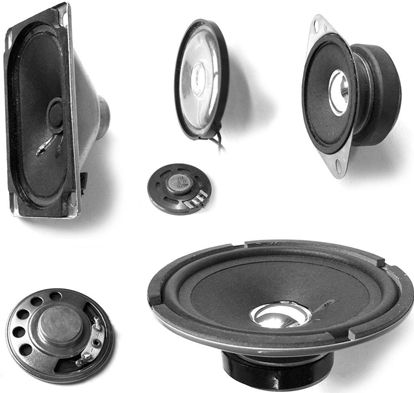
\includegraphics[width=0.6\linewidth]{Image00444}
	\caption{扬声器外形}
	\label{fig:speaker_shapes}
\end{figure}

\subsection{扬声器的种类}

扬声器按换能方式可分为电动式扬声器、舌簧式扬声器、压电式扬声器和气动式扬声器等，按结构可分为纸盆式扬声器、球顶式扬声器、号筒式扬声器、带式扬声器和平板式扬声器等，按照工作频率范围可分为高音扬声器、中音扬声器、低音扬声器和全频扬声器等。

\subsection{扬声器的符号}

扬声器的文字符号是"BL"，图形符号如图4-2所示。

\begin{figure}[htbp]
	\centering
	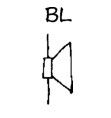
\includegraphics[width=0.3\linewidth]{Image00448}
	\caption{扬声器的图形符号}
	\label{fig:speaker_symbols}
\end{figure}

\subsection{扬声器的型号}

扬声器的型号命名由4个部分组成。第一部分用字母"Y"表示扬声器的主称，第二部分用字母表示扬声器的类型，第三部分用字母或数字表示扬声器的额定功率或口径等特征，第四部分用数字表示序号。

\subsection{扬声器的参数}

扬声器的主要参数有额定功率、标称阻抗、频率范围和灵敏度等。

\subsubsection{1．额定功率}

额定功率是指扬声器能够长期正常工作的输入电功率。

\subsubsection{2．标称阻抗}

标称阻抗是指扬声器在特定频率下的交流阻抗值。

\subsubsection{3．频率范围}

频率范围是指扬声器能够有效重放的频率范围。

\subsubsection{4．灵敏度}

灵敏度是指扬声器在输入一定功率时产生的声压级。

\section{耳机}

耳机也是常用的电声转换器件，主要用于个人聆听。常见耳机如图4-11所示。

\begin{figure}[htbp]
	\centering
	
\includegraphics[width=0.6\linewidth]{Image00210}
	\caption{耳机外形}
	\label{fig:headphone_shapes}
\end{figure}

\subsection{耳机的种类}

耳机按结构形式可分为头戴式、耳挂式、耳塞式、听诊式和手持式等，按传送声音的不同可分为单声道耳机和立体声耳机两种，按换能方式的不同可分为电动式、电磁式、压电式、静电式、平膜式、平板式等。

\subsection{耳机的符号}

耳机的文字符号是"BE"，图形符号如图4-12所示。

\begin{figure}[htbp]
	\centering
	
\includegraphics[width=0.3\linewidth]{Image00212}
	\caption{耳机的图形符号}
	\label{fig:headphone_symbols}
\end{figure}

\subsection{耳机的型号}

耳机的型号命名由4个部分组成。第一部分用字母"E"表示耳机的主称，第二部分用字母表示耳机的类型，第三部分用字母或数字表示耳机的特征，第四部分用数字表示序号。

耳机型号中字母代号的含义见表4-2。例如：型号为EDL-3表示这是立体声动圈式耳机，型号为ECS-1表示这是电磁式耳塞机。

\subsection{耳机的参数}

耳机的主要参数有标称阻抗、频率范围和灵敏度等，耳机有低阻和高阻之分。

\subsubsection{1．标称阻抗}

标称阻抗是指耳机在特定频率下的交流阻抗值。

\subsubsection{2．频率范围}

频率范围是指耳机能够有效重放的频率范围。

\subsubsection{3．灵敏度}

灵敏度是指耳机在输入一定功率时产生的声压级。

\section{传声器}

传声器是将声能转换为电能的元件，俗称麦克风。

\subsection{传声器的种类}

传声器按工作原理可分为：

\begin{itemize}[leftmargin=2cm]
	\item \textbf{动圈式传声器}：利用电磁感应原理
	\item \textbf{电容式传声器}：利用电容变化原理
	\item \textbf{驻极体传声器}：利用驻极体材料
\end{itemize}

\section{电磁讯响器}

电磁讯响器是一种常用的电声转换器件，用于发出声音信号。

\subsection{电磁讯响器的种类}

电磁讯响器按工作原理可分为：

\begin{itemize}[leftmargin=2cm]
	\item \textbf{不带音源讯响器}：需要外部驱动信号
	\item \textbf{自带音源讯响器}：内置振荡电路
\end{itemize}

\subsection{电磁讯响器的符号}

电磁讯响器的文字符号为"HA"，图形符号与扬声器类似。

\subsection{电磁讯响器的参数}

电磁讯响器的主要参数有额定电压、工作电流和发声频率。

\subsection{电磁讯响器的特点}

电磁讯响器具有体积小、功耗低、声音清晰的特点。

\subsection{不带音源讯响器}

不带音源讯响器需要外部驱动信号才能发声，具有频率可调的特点。

\subsection{自带音源讯响器}

自带音源讯响器内置振荡电路，接通电源即可发声，使用方便。

\section{压电蜂鸣器}

压电蜂鸣器是利用压电效应发声的电声转换器件。

\subsection{压电蜂鸣器的符号}

压电蜂鸣器的文字符号为"HA"，图形符号与电磁讯响器类似。

\subsection{压电蜂鸣器的工作原理}

压电蜂鸣器利用压电陶瓷的逆压电效应，在电场作用下产生机械振动而发声。

\subsection{压电蜂鸣器的特点}

压电蜂鸣器具有功耗低、体积小、可靠性高的特点。

\subsection{压电蜂鸣器的作用}

压电蜂鸣器主要用于报警、提示和信号发声等应用。

\section{传声器的详细内容}

传声器是将声能转换为电能的元件，俗称麦克风。

\subsection{传声器的种类}

传声器按工作原理可分为：

\begin{itemize}[leftmargin=2cm]
	\item \textbf{动圈式传声器}：利用电磁感应原理
	\item \textbf{电容式传声器}：利用电容变化原理
	\item \textbf{驻极体传声器}：利用驻极体材料
	\item \textbf{近讲传声器}：适合近距离使用
	\item \textbf{无线传声器}：无需连接线缆
\end{itemize}

\subsection{传声器的符号}

传声器的文字符号为"BM"，图形符号如图4-20所示。

\subsection{传声器的型号}

传声器的型号命名由4个部分组成，第一部分用字母"C"表示传声器。

\subsection{传声器的参数}

传声器的主要参数有灵敏度、频率响应和指向性等。

\subsection{动圈式传声器}

动圈式传声器利用电磁感应原理，具有结构简单、可靠性高的特点。

\subsection{驻极体传声器}

驻极体传声器利用驻极体材料，具有灵敏度高、体积小的特点。

\subsection{近讲传声器}

近讲传声器适合近距离使用，具有抗干扰能力强的特点。

\subsection{无线传声器}

无线传声器无需连接线缆，使用方便灵活。

\section{晶体}

石英晶体谐振器通常简称为晶体，是一种常用的选择频率和稳定频率的电子元件，广泛应用在电子仪器仪表、通信设备、广播和电视设备、影音播放设备、计算机以及电子钟表等领域。

\subsection{晶体的种类}

晶体一般密封在金属、玻璃或塑料等外壳中。晶体按频率稳定度可分为普通型和高精度型，其标称频率和体积大小也有多种规格。

\subsection{晶体的符号}

晶体的文字符号为"B"或"BC"，图形符号如图4-44所示。

\subsection{晶体的参数}

晶体的主要参数有标称频率、负载电容和激励电平等。

\subsubsection{1．标称频率}

标称频率是指晶体在特定条件下能够产生的谐振频率。

\subsubsection{2．负载电容}

负载电容是指晶体正常工作时需要的外部电容值。

\subsubsection{3．激励电平}

激励电平是指晶体正常工作时需要的激励功率。

\subsection{晶体的特点}

晶体的特点是具有压电效应，可等效为一个品质因数极高的谐振回路。

\subsection{晶体的作用}

晶体的作用是构成频率稳定度很高的振荡器。

\chapter{第5章 控制与保护器件}

控制与保护器件主要包括继电器、开关、接插件和保险器件等，是电子电路中经常使用的器件。

\section{继电器}

继电器是一种常用的控制器件，它可以用较小的电流来控制较大的电流，用低电压来控制高电压，用直流电来控制交流电等，并且可实现控制电路与被控电路之间的完全隔离，在自动控制、遥控、保护电路等方面得到广泛的应用。

\begin{figure}[htbp]
	\centering
	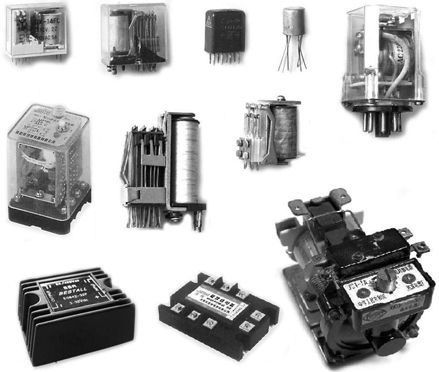
\includegraphics[width=0.6\linewidth]{Image00507}
	\caption{继电器外形}
	\label{fig:relay_shapes}
\end{figure}

\subsection{继电器的种类}

继电器的种类很多，外形各异。继电器根据结构与特征可分为电磁式继电器、干簧式继电器、湿簧式继电器、压电式继电器、固态继电器、磁保持继电器、步进继电器、时间继电器、温度继电器等。

按照工作电压类型的不同，继电器可分为直流型继电器、交流型继电器和脉冲型继电器。

按照继电器触点的形式与数量，可分为单组触点继电器和多组触点继电器两类。其中单组触点继电器又分为常开触点（动合触点，简称H触点）、常闭触点（动断触点，简称D触点）、转换触点（简称Z触点）3种；多组触点继电器既可以包括多组相同形式的触点，又可以包括多种不同形式的触点。

\subsection{继电器的符号}

继电器的文字符号为"K"，图形符号如图5-2所示。在电路图中，继电器的触点可以画在该继电器线圈的旁边，也可以为了便于图面布局将触点画在远离该继电器线圈的地方，而用编号表示它们是一个继电器。

\begin{figure}[htbp]
	\centering
	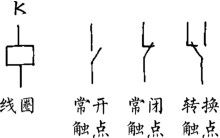
\includegraphics[width=0.4\linewidth]{Image00512}
	\caption{继电器的图形符号}
	\label{fig:relay_symbols}
\end{figure}

\subsection{继电器的型号}

继电器的型号命名一般由5个部分组成。第一部分用字母"J"表示继电器的主称，第二部分用字母表示继电器的功率或形式，第三部分用字母表示继电器的外形特征，第四部分用1～2位数字表示序号，第五部分用字母表示继电器的封装形式。

继电器型号中字母代号的含义见表 5-1。例如：型号为JZX-10M表示这是中功率小型密封式电磁继电器，型号为JAG-2表示这是干簧式继电器。

\subsection{继电器的参数}

继电器的主要参数有额定工作电压、额定工作电流、线圈电阻和触点负荷等。继电器各参数可通过查看说明书或手册得知。

\subsubsection{1．额定工作电压}

额定工作电压是指继电器正常工作时线圈需要的电压值，对于直流继电器是指直流电压值，对于交流继电器则是指交流电压值。同一种型号的继电器往往有多种额定工作电压以供选择，并在型号后面加以规格号来区别。

\subsubsection{2．额定工作电流}

额定工作电流是指继电器正常工作时线圈需要的电流值，对于直流继电器是指直流电流值，对于交流继电器则是指交流电流值。选用继电器时必须保证其额定工作电压和额定工作电流符合要求。

\subsubsection{3．线圈电阻}

线圈电阻是指继电器线圈的直流电阻。对于直流继电器，线圈电阻与额定工作电压和额定工作电流的关系符合欧姆定律。

\subsubsection{4．触点负荷}

触点负荷是指继电器触点的负载能力，也称为触点容量。例如：JZX-10M型继电器的触点负荷为直流28V×2A或交流115V×1A。使用中通过继电器触点的电压、电流均不应超过规定值，否则会烧坏触点，造成继电器损坏。一个继电器的多组触点的负荷一般都是一样的。

\subsection{继电器的作用}

继电器的主要作用是间接控制和隔离控制。

\subsubsection{1．间接控制}

继电器用于声控电灯开关，这是弱电控制强电的典型例子。当传声器BM接收到声音信号时，该信号经放大后使继电器K吸合，其触点接通照明灯的市电电源使其点亮。

\subsubsection{2．隔离控制}

继电器用于扬声器保护电路，这是隔离控制的典型例子。功率放大器L声道或R声道的输出端如果出现直流电压，被扬声器保护电路检测放大后，使继电器吸合，其触点断开，切断了功放输出端与扬声器的连接，保护了扬声器免予被烧毁。采用继电器控制扬声器的通断，使保护电路与音频电路完全隔离，确保了高保真的音质。

\subsubsection{3．保护二极管的作用}

由于继电器线圈实质上是一个大电感，为避免驱动继电器的晶体管被损坏，实际使用中应在继电器线圈两端并接保护二极管。当开关管关断的瞬间，继电器线圈产生的反向高压可以通过保护二极管泄放，保护了开关管不会被反向高压所击穿。

\section{开关}

开关是控制电路通断的元件。

\subsection{开关的种类}

开关按操作方式可分为：

\begin{itemize}[leftmargin=2cm]
	\item \textbf{拨动开关}：通过拨动操作
	\item \textbf{按钮开关}：通过按压操作
	\item \textbf{旋转开关}：通过旋转操作
	\item \textbf{微动开关}：通过微小位移操作
	\item \textbf{轻触开关}：通过轻触操作
	\item \textbf{薄膜开关}：通过薄膜按压操作
\end{itemize}

\subsection{开关的符号}

开关的文字符号为"S"，图形符号根据开关类型有所不同。

\subsection{开关的参数}

开关的主要参数有额定电压、额定电流、接触电阻和机械寿命等。

\subsection{拨动开关}

拨动开关通过拨动操作杆实现电路通断，具有结构简单、可靠性高的特点。

\subsection{旋转开关}

旋转开关通过旋转操作轴实现多路切换，适用于多档位选择电路。

\subsection{按钮开关}

按钮开关通过按压操作实现电路通断，分为常开型和常闭型两种。

\subsection{微动开关和轻触开关}

微动开关和轻触开关通过微小位移操作，具有灵敏度高、体积小的特点。

\subsection{薄膜开关}

薄膜开关采用薄膜结构，具有防水、防尘、美观的特点。

\section{保险丝}

保险丝是电路过流保护元件。

\subsection{保险丝的种类}

保险丝按结构可分为：

\begin{itemize}[leftmargin=2cm]
	\item \textbf{玻璃管保险丝}：熔丝封装在玻璃管内
	\item \textbf{陶瓷保险丝}：熔丝封装在陶瓷管内
	\item \textbf{自恢复保险丝}：过流后可自动恢复
	\item \textbf{快速熔断保险丝}：快速响应过流
	\item \textbf{延时熔断保险丝}：允许短暂过流
\end{itemize}

\subsection{保险丝的符号}

保险丝的文字符号为"F"，图形符号如图5-40所示。

\subsection{保险丝的参数}

保险丝的主要参数有额定电流、额定电压和分断能力等。

\subsection{保险丝的工作原理}

保险丝利用金属熔丝在过流时发热熔断的原理，保护电路免受过流损坏。

\subsection{常用保险丝}

常用保险丝包括普通玻璃管保险丝、陶瓷保险丝和自恢复保险丝等。

\section{接插件}

接插件是实现电路器件、部件或组件之间可拆卸连接的连接器件，包括各种插头、插座与接线端子等。

\subsection{接插件的种类}

接插件的种类很多，大小各异。接插件按形式可分为单芯插头/插座、二芯插头/插座、三芯插头/插座、同轴插头/插座和多极插头/插座等，按用途可分为音视频插头/插座、印制电路板插座、电源插头/插座、集成电路插座、管座、接线柱、接线端子和连接器等。

\begin{figure}[htbp]
	\centering
	
\includegraphics[width=0.6\linewidth]{Image00093}
	\caption{接插件外形}
	\label{fig:connectors_shapes}
\end{figure}

\subsection{接插件的符号}

接插件的一般文字符号为"X"，插头的文字符号为"XP"，插座的文字符号为"XS"，它们的图形符号如图5-36所示。

\begin{figure}[htbp]
	\centering
	
\includegraphics[width=0.4\linewidth]{Image00092}
	\caption{接插件的图形符号}
	\label{fig:connectors_symbols}
\end{figure}

\subsection{常用接插件}

常用接插件主要有二芯插头/插座、三芯插头/插座和同轴插头/插座等。

\subsubsection{1．二芯插头/插座}

二芯插头/插座常用的规格有2.5mm、3.5mm、6.35mm（指插头的外直径）等，大都兼有转换开关功能，主要应用于音频信号的连接和转接。音响设备的传声器和耳机一般采用 6.35mm 的插头/插座，袖珍型收音机等通常采用2.5mm或3.5mm的插头/插座。

图5-37所示为收音机外接耳机电路。耳机插头未插入时，插座XS的a端与b端连通，扬声器BL发声。当耳机插头插入后，插座XS的a端被插头顶开脱离b端，使扬声器BL停止发声而改由耳机发声。

\begin{figure}[htbp]
	\centering
	
\includegraphics[width=0.6\linewidth]{Image00096}
	\caption{二芯插头/插座的应用}
	\label{fig:two_pin_connector_application}
\end{figure}

\subsubsection{2．三芯插头/插座}

三芯插头/插座的规格和转换功能等均与二芯插头/插座一样，主要用于立体声音频信号的连接和转接。

图 5-38 所示为立体声收音机外接耳机电路。耳机插头未插入时，插座XS的a端与b端、c端与d端连通，左、右声道扬声器BL$_1$、BL$_2$发声。当耳机插头插入后，插座XS的a端和c端分别与b端和d端脱离，而与耳机连通，使扬声器停止发声而改由耳机发声。

\begin{figure}[htbp]
	\centering
	
\includegraphics[width=0.6\linewidth]{Image00069}
	\caption{三芯插头/插座的应用}
	\label{fig:three_pin_connector_application}
\end{figure}

\subsubsection{3．同轴插头/插座}

同轴插头/插座结构如图5-39所示，信号线在中心，地线在周围，并采用屏蔽线连接。同轴插头/插座主要用于电视机、录像机、调谐器、放大器、CD和DVD等音视频信号的输入、输出连接。

\begin{figure}[htbp]
	\centering
	
\includegraphics[width=0.3\linewidth]{Image00072}
	\caption{同轴插头/插座结构}
	\label{fig:coaxial_connector_structure}
\end{figure}

\chapter{第6章 晶体二极管与单结晶体管}

晶体二极管是电子电路中最重要的半导体器件，包括一般二极管和特殊二极管两大类。单结晶体管也是一种特殊的半导体二极管。

\section{晶体二极管}

晶体二极管简称二极管，是一种常用的具有一个PN结的半导体器件。

\begin{figure}[htbp]
	\centering
	
\includegraphics[width=0.6\linewidth]{Image00065}
	\caption{晶体二极管外形}
	\label{fig:diode_shapes}
\end{figure}

\subsection{晶体二极管的种类}

晶体二极管品种很多，大小各异，仅从外观上看，较常见的有玻璃壳二极管、塑封二极管、金属壳二极管、大功率螺栓状金属壳二极管、微型二极管、片状二极管等。

晶体二极管按制造材料的不同，可分为锗管和硅管两大类，每一类又分为N型和P型；按制造工艺不同，可分为点接触型二极管和面接触型二极管。

晶体二极管按功能与用途不同，可分为一般二极管和特殊二极管两大类。一般二极管包括检波二极管、整流二极管、开关二极管等。特殊二极管主要有稳压二极管、敏感二极管（磁敏二极管、温度效应二极管、压敏二极管等）、变容二极管、发光二极管、光电二极管、激光二极管等。没有特别说明时，晶体二极管即指一般二极管。

\subsection{晶体二极管的符号}

晶体二极管的文字符号是"VD"，图形符号如图6-2所示。

\begin{figure}[htbp]
	\centering
	
\includegraphics[width=0.2\linewidth]{Image00087}
	\caption{晶体二极管的图形符号}
	\label{fig:diode_symbols}
\end{figure}

\subsection{晶体二极管的型号}

晶体二极管的型号命名一般由5个部分组成。第一部分用数字"2"表示二极管，第二部分用字母表示材料和极性，第三部分用字母表示类型，第四部分用数字表示序号，第五部分用字母表示规格。

\subsection{晶体二极管的参数}

晶体二极管的主要参数有最大整流电流、最大反向电压和最高工作频率。

\subsubsection{1．最大整流电流}

最大整流电流是指二极管长期正常工作时，允许通过的最大正向平均电流值。

\subsubsection{2．最大反向电压}

最大反向电压是指二极管正常工作时所能承受的最大反向电压值。

\subsubsection{3．最高工作频率}

最高工作频率是指二极管正常工作时的最高频率。

\subsection{晶体二极管的特点}

晶体二极管的特点是具有单向导电特性，即电流只能从正极流向负极，而不能从负极流向正极。

\subsection{晶体二极管的作用}

晶体二极管的主要作用是整流、检波和开关。

\subsubsection{1．整流}

将交流电转换为直流电。

\subsubsection{2．检波}

从调制信号中检出调制信号。

晶体管收音机中常用2AP系列型号的二极管作检波二极管。其中2AP9和2AP10效果更好些，也可以用2AK型的二极管。某些2CP型的二极管(如2CP10)的外形与2AP型差不多，但这类二极管的工作频率低、极间电容大，起始电压高，是不能用来担任检波的，不能认错或调换，这一点希望能引起注意。

\subsubsection{3．开关}

在数字电路中用作电子开关。

\section{稳压二极管}

稳压二极管是一种特殊的晶体二极管，用于稳定电压。

\subsection{稳压二极管的种类}

稳压二极管按结构可分为普通稳压二极管和温度补偿型稳压二极管两大类。

\subsection{稳压二极管的符号}

稳压二极管的文字符号为"VD"，图形符号与普通二极管相似，但在符号上标有稳压值。

\subsection{稳压二极管的极性}

稳压二极管的正负极性与普通二极管相同，即带色环的一端为负极。

\subsection{稳压二极管的参数}

稳压二极管的主要参数有稳定电压、稳定电流和最大耗散功率等。

\subsection{稳压二极管的特点与工作原理}

稳压二极管利用PN结的反向击穿特性来稳定电压。当反向电压达到击穿电压时，电流急剧增大而电压基本保持不变。

\subsection{稳压二极管的作用}

稳压二极管主要用于电源电路中的电压稳定，也可用作基准电压源和过压保护。

\subsection{特殊稳压二极管}

特殊稳压二极管包括双向稳压二极管、温度补偿稳压二极管等，具有特殊的稳压特性。

\section{单结晶体管}

单结晶体管是具有负阻特性的半导体器件。

\subsection{单结晶体管的应用}

单结晶体管主要用于振荡电路和定时电路。

\chapter{第7章 晶体三极管与晶闸管}

晶体三极管（包括场效应管）是具有放大作用的半导体器件，是电子电路中的核心器件之一。晶闸管是一种功率型半导体器件，在各种控制电路中的应用十分广泛。

\section{晶体三极管}

晶体三极管通常简称为晶体管或三极管，是一种具有两个PN结的半导体器件。晶体三极管是最重要的电子元器件之一，在电子电路中起着核心的作用。

三极管在电路中用字母VT表示（传统表示方法中曾使用BG）。晶体三极管有三条引线(也叫管脚)，是它的三个电极，分别叫做发射极、基极和集电极，各自用字母e、b和c表示。根据制造材料和构造的不同，常用的晶体三极管分锗管和硅管两类，每类又分PNP型和NPN型两种。同时，根据工作频率的高低，三极管还分高频管和低频管。

\begin{figure}[htbp]
	\centering
	
\includegraphics[width=0.6\linewidth]{Image00374}
	\caption{晶体三极管外形}
	\label{fig:transistor_shapes}
\end{figure}

\subsection{晶体三极管的种类}

晶体三极管的种类繁多，形状和大小各不相同。

（1）按所用半导体材料的不同，晶体三极管可分为锗管、硅管和化合物管。

（2）按导电极性不同，晶体三极管可分为NPN型晶体三极管和PNP型晶体三极管两大类。NPN型晶体三极管工作时，集电极c和基极b接正电压，电流由集电极c和基极b流向发射极e。PNP型晶体三极管工作时，集电极c和基极b接负电压，电流由发射极e流向集电极c和基极b。

（3）晶体三极管按截止频率可分为超高频管、高频管（≥3MHz）和低频管（＜3MHz），按耗散功率可分为小功率管（＜1W）和大功率管（≥1W），按用途可分为低频放大管、高频放大管、开关管、低噪声管、高反压管、复合管等。

\subsection{晶体三极管的符号}

晶体三极管的文字符号为"VT"，图形符号如图7-2所示。

\begin{figure}[htbp]
	\centering
	
\includegraphics[width=0.4\linewidth]{Image00376}
	\caption{晶体三极管的图形符号}
	\label{fig:transistor_symbols}
\end{figure}

\subsection{晶体三极管的型号}

国产晶体三极管的型号命名由5个部分组成。第一部分用数字"3"表示三极管，第二部分用字母表示材料和极性，第三部分用字母表示类别，第四部分用数字表示序号，第五部分用字母表示规格。

晶体三极管型号的含义见表7-1。例如：3AX31为PNP型锗材料低频小功率晶体三极管，3DG6B为NPN型硅材料高频小功率晶体三极管。

\subsection{晶体三极管的引脚}

晶体三极管有3根引脚，分别是基极b、发射极e和集电极c，使用中应识别清楚。绝大多数小功率晶体三极管的引脚均按e、b、c的标准顺序排列，并标有标志。但也有例外，如某些晶体三极管型号后有后缀"R"，其引脚排列顺序往往是e、c、b。

\subsection{晶体三极管的参数}

晶体三极管的参数很多，包括直流参数、交流参数、极限参数3类，但一般使用时只需关注电流放大倍数$\beta$、特征频率$f_T$、集-射极击穿电压$BU_{ceo}$、集电极最大电流$I_{cm}$和集电极最大功耗$P_{cm}$等。

\subsubsection{1．电流放大倍数}

电流放大倍数$\beta$表示晶体三极管的放大能力。

\subsubsection{2．特征频率}

特征频率$f_T$表示晶体三极管的频率特性。

\subsubsection{3．集-射极击穿电压}

集-射极击穿电压$BU_{ceo}$表示晶体三极管的耐压能力。

\subsubsection{4．集电极最大电流}

集电极最大电流$I_{cm}$表示晶体三极管的电流承受能力。

\subsubsection{5．集电极最大功耗}

集电极最大功耗$P_{cm}$表示晶体三极管的功率承受能力。

\subsection{晶体三极管的特点}

晶体三极管的特点是具有电流放大作用，是电流控制型器件。

\subsection{晶体三极管的作用}

晶体三极管的主要作用是放大、振荡、电子开关、可变电阻和阻抗变换。

\subsubsection{1．放大}

晶体三极管可以将微弱的电信号放大。

\subsubsection{2．振荡}

晶体三极管可以组成各种振荡电路。

\subsubsection{3．电子开关}

晶体三极管在数字电路中用作电子开关。

\subsubsection{4．可变电阻}

晶体三极管可以工作在可变电阻状态。

\subsubsection{5．阻抗变换}

晶体三极管可以实现阻抗变换功能。

\subsection{晶体三极管的应用指导}

单管机最常用的是3AG系列型号的三极管。如3AG1、3AG11、3AG44等，3AK9、3AK10等也可以代用。它们都是PNP型高频管。有的单管机电路也使用3DG6或3KD2等NPN型硅高频管。目前大多数锗三极管是PNP型管，但也有少数是NPN型管，如3BX31等；大多数硅管是NPN型管，但也有少数是PNP型管，如3CG21等。

\section{场效应管}

场效应管是一种电压控制型半导体器件，具有输入阻抗高、噪声低、热稳定性好等优点。

\subsection{场效应管的种类}

场效应管按结构可分为结型场效应管和绝缘栅型场效应管两大类。

\subsection{场效应管的符号}

场效应管的文字符号为"VT"，图形符号根据类型不同而有所区别。

\subsection{场效应管的引脚}

场效应管一般有三个引脚：源极（S）、栅极（G）和漏极（D）。

\subsection{场效应管的参数}

场效应管的主要参数有夹断电压、饱和漏电流、跨导和最大耗散功率等。

\subsection{场效应管的特点与工作原理}

场效应管利用栅极电压控制沟道导电能力，实现信号放大。

\subsection{场效应管的作用}

场效应管主要用于放大电路、开关电路和高频电路。

\subsection{常用场效应管}

常用场效应管包括小功率场效应管、功率场效应管和射频场效应管等。

\section{晶闸管}

晶闸管是具有可控整流特性的半导体器件。

\subsection{晶闸管的种类}

晶闸管按结构可分为：

\begin{itemize}[leftmargin=2cm]
	\item \textbf{单向晶闸管}：单向导通
	\item \textbf{双向晶闸管}：双向导通
\end{itemize}

\subsection{晶闸管的特点}

晶闸管的特点是具有可控整流特性，可以通过控制极信号来控制导通。

\subsection{晶闸管的作用}

晶闸管主要用于功率控制和调节电路。

\chapter{第8章 光电器件}

光电器件是指能够将光信号转换为电信号的半导体器件，包括光电二极管、光电三极管和光电耦合器等。

\section{光电二极管}

光电二极管是一种常用的光敏器件，和晶体二极管相似，光电二极管也是具有一个PN结的半导体器件，不同的是光电二极管有一个透明的窗口，以便使光线能够照射到PN结上。

\begin{figure}[htbp]
	\centering
	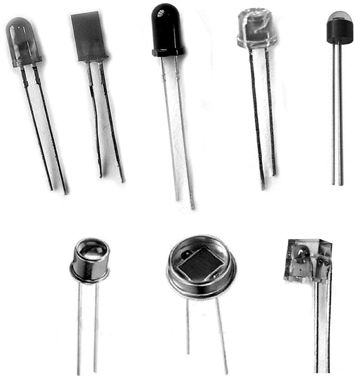
\includegraphics[width=0.6\linewidth]{Image00459}
	\caption{光电二极管外形}
	\label{fig:photodiode_shapes}
\end{figure}

\subsection{光电二极管的种类}

光电二极管有许多种类，常用的有PN结型、PIN结型、雪崩型和肖特基结型等，用得最多的是硅材料PN结型光电二极管。外形上常见的有透明塑封光电二极管、金属壳封装光电二极管、树脂封装光电二极管等。

\subsection{光电二极管的符号}

光电二极管的文字符号为"VD"，图形符号如图8-2所示。

\begin{figure}[htbp]
	\centering
	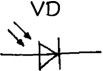
\includegraphics[width=0.2\linewidth]{Image00461}
	\caption{光电二极管的图形符号}
	\label{fig:photodiode_symbols}
\end{figure}

\subsection{光电二极管的型号}

光电二极管的型号命名一般由5个部分组成。第一部分用数字"2"表示二极管，第二部分用字母表示材料和极性，第三部分用字母表示类型，第四部分用数字表示序号，第五部分用字母表示规格。

\subsection{光电二极管的参数}

光电二极管的主要参数是最高工作电压、光电流和光电灵敏度等。

\subsubsection{1．最高工作电压}

最高工作电压是指光电二极管在无光照条件下能够承受的最大反向电压值。

\subsubsection{2．光电流}

光电流是指光电二极管在受到一定光照时产生的电流值。

\subsubsection{3．光电灵敏度}

光电灵敏度是指光电二极管对光照的敏感程度。

\subsection{光电二极管的特点}

光电二极管的特点是具有将光信号转换为电信号的功能。

\subsection{光电二极管的作用}

光电二极管的作用是进行光电转换，在光控、红外遥控、光探测、光纤通信和光电耦合等方面有广泛的应用。

\section{发光二极管}

发光二极管是将电能转换为光能的半导体器件。

\subsection{发光二极管的种类}

发光二极管按发光颜色可分为：

\begin{itemize}[leftmargin=2cm]
	\item \textbf{红色发光二极管}
	\item \textbf{绿色发光二极管}
	\item \textbf{蓝色发光二极管}
	\item \textbf{白色发光二极管}
\end{itemize}

\subsection{发光二极管的特点}

发光二极管的特点是低功耗、长寿命、响应速度快。

\subsection{发光二极管的作用}

发光二极管主要用于指示灯、显示屏、照明和光通信等应用。

\section{光电三极管}

光电三极管是具有光电转换功能的三端半导体器件。

\subsection{光电三极管的特点}

光电三极管的特点是具有电流放大功能，光电灵敏度比光电二极管高。

\subsection{光电三极管的应用}

光电三极管主要用于光检测和光电放大电路。

\section{光电耦合器}

光电耦合器是将发光器件和光敏器件集成在一起的器件。

\subsection{光电耦合器的特点}

光电耦合器的特点是实现电气隔离，提高电路的安全性。

\subsection{光电耦合器的应用}

光电耦合器主要用于隔离控制、信号传输和电平转换等应用。

\chapter{第9章 集成电路}

集成电路是高度集成化的电子器件，具有集成度高、功能完整、可靠性好、体积小、重量轻、功耗低的特点，已成为现代电子技术中不可或缺的核心器件。

集成电路可分为模拟集成电路和数字集成电路两大类，包括集成运放、时基集成电路、集成稳压器、门电路、触发器、计数器、译码器和移位寄存器等。

\section{集成运放}

集成运算放大器简称集成运放，是一种集成化的、高增益的多级直接耦合放大器，具有输入阻抗高、增益大、稳定性好、通用性强、适用范围宽和使用简便的特点，并且有很多品种可供选择，在放大、振荡、电压比较、阻抗变换、模拟运算和有源滤波等各种电子电路中得到了越来越广泛的应用。

\begin{figure}[htbp]
	\centering
	
\includegraphics[width=0.6\linewidth]{Image00316}
	\caption{集成运放外形}
	\label{fig:opamp_shapes}
\end{figure}

\subsection{集成运放的种类}

集成运放品种繁多，按类型可分为通用型运放、低功耗运放、高阻运放、高精度运放、高速运放、宽带运放、低噪声运放、高压运放，以及程控型、电流型、跨导型运放等。根据一个集成电路封装内包含运放单元的数量，集成运放又可分为单运放、双运放和四运放。

集成运放有金属圆壳封装、金属菱形封装、陶瓷扁平式封装、双列直插式封装等形式。较常用的是双列直插式封装的集成运放。

\subsection{集成运放的符号}

集成运放的文字符号为"IC"，其图形符号如图9-2所示。集成运放一般具有两个输入端，即同相输入端$U_+$和反相输入端$U_-$，以及一个输出端$U_o$。

\begin{figure}[htbp]
	\centering
	
\includegraphics[width=0.3\linewidth]{Image00318}
	\caption{集成运放的图形符号}
	\label{fig:opamp_symbols}
\end{figure}

\subsection{集成运放的参数}

集成运放的参数主要有电源电压范围、最大允许功耗、单位增益带宽、转换速率和输入阻抗等。

\subsubsection{1．电源电压范围}

电源电压范围是指集成运放正常工作时所需的电源电压范围。

\subsubsection{2．最大允许功耗}

最大允许功耗是指集成运放能够承受的最大功耗值。

\subsubsection{3．单位增益带宽}

单位增益带宽是指集成运放开环增益为1时的频率。

\subsubsection{4．转换速率}

转换速率是指集成运放输出电压的最大变化速率。

\subsubsection{5．输入阻抗}

输入阻抗是指集成运放输入端的阻抗值。

\subsection{集成运放的特点}

集成运放的特点是输入阻抗高、增益大、稳定性好、通用性强。

\subsection{集成运放的作用}

集成运放的主要作用是放大和阻抗变换，在各种放大、振荡、有源滤波、精密整流以及运算电路中得到广泛的应用。

\section{时基集成电路}

时基集成电路是能够产生精确时间延迟和振荡的集成电路。

\subsection{时基集成电路的特点}

时基集成电路的特点是能够产生精确的时间基准信号。

\subsection{时基集成电路的应用}

时基集成电路主要用于定时器、振荡器和脉冲发生器等电路。

\section{集成稳压器}

集成稳压器是能够提供稳定直流电压的集成电路。

\subsection{集成稳压器的特点}

集成稳压器的特点是输出电压稳定、使用方便。

\subsection{集成稳压器的应用}

集成稳压器主要用于电源电路中提供稳定的直流电压。

\section{数字集成电路}

数字集成电路是处理离散信号的集成电路。

\subsection{数字集成电路的种类}

数字集成电路按功能可分为：

\begin{itemize}[leftmargin=2cm]
	\item \textbf{门电路}：实现基本逻辑功能
	\item \textbf{触发器}：存储二进制信息
	\item \textbf{计数器}：实现计数功能
	\item \textbf{译码器}：实现译码功能
	\item \textbf{移位寄存器}：实现移位功能
\end{itemize}

\subsection{集成电路的封装}

集成电路的封装形式多样，常见的有：

\begin{itemize}[leftmargin=2cm]
	\item \textbf{DIP封装}：双列直插式
	\item \textbf{SOP封装}：小外形封装
	\item \textbf{QFP封装}：四方扁平封装
	\item \textbf{BGA封装}：球栅阵列封装
\end{itemize}

\part{无线电材料基础}

\chapter{导线材料}

漆包线、李兹线和丝包线是无线电设备中常用的导线材料，本章节将详细介绍这三种导线的基本特性、分类、应用以及选择原则等内容。

漆包线是现代电子设备中最常用的导线，具有良好的绝缘性能和耐热性能。李兹线是专门用于高频应用的特殊导线，通过多股细线绞合有效减小高频损耗。丝包线是早期的导线材料，在无线电发展史上占有重要地位。

通过学习本章节，读者将能够：

\begin{itemize}[leftmargin=3.5em]
    \item 理解漆包线、李兹线和丝包线的基本原理和特性
    \item 掌握各种导线的分类和规格表示方法
    \item 了解各种导线在无线电设备中的应用场景
    \item 学会根据实际需求选择合适的导线材料
\end{itemize}

\section{漆包线}

漆包线是一种在铜线表面涂覆绝缘漆的导线，广泛应用于各种电磁器件中。

\subsection{漆包线的基本特性}

漆包线是一种在铜线表面涂覆绝缘漆的导线，广泛应用于各种电磁器件中。漆包线的主要特点包括：

\begin{itemize}[leftmargin=3.5em]
    \item \textbf{绝缘性能好}：漆膜具有良好的绝缘性能，能够承受较高的电压
    \item \textbf{耐热性能好}：不同类型的漆包线具有不同的耐热等级，适应不同的工作温度
    \item \textbf{机械强度高}：漆膜具有良好的耐磨性和耐刮性
    \item \textbf{导线截面积小}：相比其他绝缘导线，漆包线的绝缘层很薄，有利于提高绕组的填充系数
    \item \textbf{易于绕制}：漆包线表面光滑，便于绕制各种形状的线圈
\end{itemize}

\subsection{漆包线的结构}

漆包线由导体和绝缘层两部分组成：

\begin{itemize}[leftmargin=3.5em]
    \item \textbf{导体}：通常为纯铜线，具有良好的导电性能。铜线的直径通常为 $0.02 \sim 5.0$ mm
    \item \textbf{绝缘层}：由各种绝缘漆涂覆而成，厚度通常为 $0.005 \sim 0.05$ mm
\end{itemize}

\subsection{漆包线的主要参数}

漆包线的主要技术参数包括：

\begin{itemize}[leftmargin=3.5em]
    \item \textbf{导体直径}：铜线的直径，单位为毫米（mm）或密耳（mil）
    \item \textbf{漆膜厚度}：绝缘层的厚度，影响绝缘性能和导线截面积
    \item \textbf{耐热等级}：漆包线能够长期工作的最高温度，分为多个等级
    \item \textbf{击穿电压}：绝缘层能够承受的最高电压
    \item \textbf{直流电阻}：单位长度的电阻值，影响导线的损耗
\end{itemize}

\subsection{漆包线的分类}

漆包线可以根据绝缘漆的类型和耐热等级进行分类：

\subsubsection{按绝缘漆类型分类}

\textbf{油性漆包线}：
\begin{itemize}[leftmargin=3.5em]
    \item 绝缘漆为天然树脂或合成树脂
    \item 耐热等级较低，通常为 A 级（$105^\circ$C）
    \item 价格低廉，应用广泛
    \item 绝缘性能和机械性能一般
\end{itemize}

应用场景：普通电机、变压器、电感器等。

\textbf{缩醛漆包线}：
\begin{itemize}[leftmargin=3.5em]
    \item 绝缘漆为聚乙烯醇缩醛树脂
    \item 耐热等级为 E 级（$120^\circ$C）
    \item 耐油性和耐溶剂性好
    \item 机械强度较高
\end{itemize}

应用场景：油浸变压器、电机等。

\textbf{聚氨酯漆包线}：
\begin{itemize}[leftmargin=3.5em]
    \item 绝缘漆为聚氨酯树脂
    \item 耐热等级为 B 级（$130^\circ$C）或 F 级（$155^\circ$C）
    \item 可焊性好，无需去除绝缘层即可焊接
    \item 高频性能好，介质损耗小
\end{itemize}

应用场景：高频变压器、电感器、电子设备等。

\textbf{聚酯漆包线}：
\begin{itemize}[leftmargin=3.5em]
    \item 绝缘漆为聚酯树脂
    \item 耐热等级为 B 级（$130^\circ$C）或 F 级（$155^\circ$C）
    \item 绝缘性能好，击穿电压高
    \item 机械强度高，耐磨性好
    \item 价格适中，性价比高
\end{itemize}

应用场景：变压器、电机、电感器等。

\textbf{聚酯亚胺漆包线}：
\begin{itemize}[leftmargin=3.5em]
    \item 绝缘漆为聚酯亚胺树脂
    \item 耐热等级为 H 级（$180^\circ$C）
    \item 耐热性能优异
    \item 绝缘性能和机械性能好
    \item 价格较高
\end{itemize}

应用场景：高温电机、变压器、特种电器等。

\textbf{聚酰胺酰亚胺漆包线}：
\begin{itemize}[leftmargin=3.5em]
    \item 绝缘漆为聚酰胺酰亚胺树脂
    \item 耐热等级为 C 级（$200^\circ$C以上）
    \item 耐热性能极佳
    \item 耐化学腐蚀性好
    \item 价格昂贵
\end{itemize}

应用场景：航空、航天、特种电器等。

\subsubsection{按耐热等级分类}

漆包线按耐热等级可分为以下几类：

\begin{itemize}[leftmargin=3.5em]
    \item \textbf{A级}：$105^\circ$C，油性漆，普通电机、变压器
    \item \textbf{E级}：$120^\circ$C，缩醛漆，油浸变压器、电机
    \item \textbf{B级}：$130^\circ$C，聚氨酯、聚酯漆，通用电子设备
    \item \textbf{F级}：$155^\circ$C，聚酯漆，高温环境应用
    \item \textbf{H级}：$180^\circ$C，聚酯亚胺漆，高温电机、变压器
    \item \textbf{C级}：$200^\circ$C以上，聚酰胺酰亚胺漆，特种应用
\end{itemize}

\section{李兹线}

李兹线是一种由多股细导线绞合而成的特殊导线，专门用于高频应用。

\subsection{李兹线的基本特性}

李兹线通过多股细导线绞合，有效减小高频电流的集肤效应，具有以下特点：

\begin{itemize}[leftmargin=3.5em]
    \item \textbf{高频性能好}：有效减小集肤效应，降低高频损耗
    \item \textbf{柔韧性好}：多股细线结构使导线更加柔软
    \item \textbf{可靠性高}：单根导线断裂不影响整体导电性能
    \item \textbf{成本较高}：制造工艺复杂，成本相对较高
\end{itemize}

\subsection{李兹线的结构}

李兹线由多股绝缘细导线绞合而成：

\begin{itemize}[leftmargin=3.5em]
    \item \textbf{股数}：通常为7股、19股、37股等，股数越多高频性能越好
    \item \textbf{导线直径}：单股导线直径通常为 $0.02 \sim 0.1$ mm
    \item \textbf{绞合方式}：采用特定的绞合节距和方向
    \item \textbf{绝缘层}：每股导线表面都有绝缘漆
\end{itemize}

\subsection{李兹线的主要参数}

李兹线的主要技术参数包括：

\begin{itemize}[leftmargin=3.5em]
    \item \textbf{总截面积}：所有股线截面积之和
    \item \textbf{股数}：导线的股数，影响高频性能
    \item \textbf{绞合节距}：绞合的节距长度，影响柔韧性
    \item \textbf{高频电阻}：在高频条件下的等效电阻
    \item \textbf{品质因数}：衡量高频性能的重要指标
\end{itemize}

\section{丝包线}

丝包线是早期无线电设备中常用的导线，在无线电发展史上具有重要地位。

\subsection{丝包线的基本特性}

丝包线采用天然丝或人造丝作为绝缘材料，具有以下特点：

\begin{itemize}[leftmargin=3.5em]
    \item \textbf{绝缘性能适中}：丝质绝缘层提供基本的绝缘保护
    \item \textbf{耐热性一般}：耐热温度较低，通常不超过$100^\circ$C
    \item \textbf{机械强度有限}：丝质材料耐磨性较差
    \item \textbf{历史意义重要}：在早期无线电发展中广泛应用
\end{itemize}

\subsection{丝包线的应用}

丝包线主要应用于以下场景：

\begin{itemize}[leftmargin=3.5em]
    \item \textbf{早期收音机}：20世纪上半叶的无线电设备
    \item \textbf{教学实验}：无线电技术教学和实验
    \item \textbf{复古设备}：复古无线电设备的修复和复制
    \item \textbf{特殊应用}：对绝缘材料有特殊要求的场合
\end{itemize}

\chapter{磁性材料}

磁性材料在无线电设备中具有重要应用，主要用于变压器、电感器、天线等部件。

\section{软磁材料}

软磁材料具有高磁导率和低矫顽力，适用于交变磁场应用：

\begin{itemize}[leftmargin=3.5em]
    \item \textbf{硅钢片}：电力变压器和电机铁芯
    \item \textbf{坡莫合金}：高磁导率，用于精密变压器
    \item \textbf{铁氧体}：高频应用，损耗小，用于高频变压器
    \item \textbf{非晶合金}：低损耗，用于高效变压器
\end{itemize}

\section{硬磁材料}

硬磁材料具有高矫顽力和高剩磁，适用于永磁体应用：

\begin{itemize}[leftmargin=3.5em]
    \item \textbf{铝镍钴}：早期永磁材料，温度稳定性好
    \item \textbf{铁氧体永磁}：成本低，广泛用于电机和扬声器
    \item \textbf{钕铁硼}：高磁能积，现代高性能永磁材料
    \item \textbf{钐钴}：高温性能好，用于特殊环境
\end{itemize}

\chapter{绝缘材料}

绝缘材料在无线电设备中用于电气隔离和机械支撑：

\section{有机绝缘材料}

\begin{itemize}[leftmargin=3.5em]
    \item \textbf{塑料}：PVC、PE、PP等，用于线缆绝缘
    \item \textbf{橡胶}：天然橡胶、硅橡胶，用于柔性绝缘
    \item \textbf{树脂}：环氧树脂、聚酯树脂，用于封装
    \item \textbf{纸材}：绝缘纸，用于变压器绝缘
\end{itemize}

\section{无机绝缘材料}

\begin{itemize}[leftmargin=3.5em]
    \item \textbf{陶瓷}：氧化铝、氮化铝，用于高频绝缘
    \item \textbf{玻璃}：玻璃纤维，用于高温绝缘
    \item \textbf{云母}：天然云母，用于高温高压绝缘
    \item \textbf{石棉}：早期绝缘材料，现已较少使用
\end{itemize}

\chapter{电容材料}

电容是无线电设备中不可或缺的重要电子元件，本章节将详细介绍电容的基本特性、分类、应用以及选择原则等内容。

电容作为储能和滤波的关键元件，在无线电电路中发挥着重要作用。从高频谐振电路到电源滤波电路，从信号耦合到定时控制，电容都是不可或缺的基础元件。

通过学习本章节，读者将能够：

\begin{itemize}[leftmargin=3.5em]
    \item 理解电容的基本原理和工作特性
    \item 掌握各类电容的分类和技术特点
    \item 了解电容在无线电电路中的应用场景
    \item 学会根据电路需求选择合适的电容类型
\end{itemize}

\section{电容的基本概念}

\subsection{电容的定义与特性}

电容是电子电路中用于存储电荷的无源元件，其基本定义基于电荷存储能力。电容的物理定义可以用以下公式表示：

\[ C = \frac{Q}{V} \]

其中：
\begin{itemize}[leftmargin=3.5em]
    \item $C$：电容值，单位为法拉（F）
    \item $Q$：存储的电荷量，单位为库仑（C）
    \item $V$：电容器两端的电压，单位为伏特（V）
\end{itemize}

电容的基本特性包括：
\begin{itemize}[leftmargin=3.5em]
    \item \textbf{电荷存储}：能够存储和释放电荷
    \item \textbf{电压滞后}：电压变化滞后于电流变化
    \item \textbf{频率特性}：阻抗随频率变化而变化
    \item \textbf{能量存储}：能够存储电场能量
\end{itemize}

\subsection{电容的结构与参数}

电容的基本结构由两个导体极板和中间的绝缘介质组成：

\textbf{基本结构组成}：
\begin{itemize}[leftmargin=3.5em]
    \item \textbf{电极板}：通常为金属箔或金属化薄膜
    \item \textbf{介质层}：绝缘材料，决定电容的主要特性
    \item \textbf{引出端}：连接电极板与外部电路的端子
    \item \textbf{封装外壳}：保护内部结构，提供机械支撑
\end{itemize}

\textbf{主要技术参数}：

\textbf{基本参数}：
\begin{itemize}[leftmargin=3.5em]
    \item \textbf{电容值}：存储电荷的能力，单位法拉（F）
    \item \textbf{额定电压}：能够长期安全工作的最高电压
    \item \textbf{容差}：实际电容值与标称值的允许偏差
    \item \textbf{温度系数}：电容值随温度变化的程度
\end{itemize}

\textbf{性能参数}：
\begin{itemize}[leftmargin=3.5em]
    \item \textbf{等效串联电阻（ESR）}：电容的等效电阻，影响高频性能
    \item \textbf{损耗角正切（tanδ）}：衡量电容能量损耗的参数
    \item \textbf{绝缘电阻}：介质绝缘性能的指标
    \item \textbf{自谐振频率}：电容与寄生电感谐振的频率
\end{itemize}

\textbf{可靠性参数}：
\begin{itemize}[leftmargin=3.5em]
    \item \textbf{寿命}：在额定条件下的使用寿命
    \item \textbf{耐压强度}：能够承受的瞬时过电压能力
    \item \textbf{温度范围}：能够正常工作的温度范围
    \item \textbf{可靠性指标}：失效率、平均无故障时间等
\end{itemize}

\section{电容的分类与应用}

\subsection{陶瓷电容}

陶瓷电容是以陶瓷材料作为介质的电容器，具有体积小、成本低、频率特性好等优点：

\textbf{主要类型}：
\begin{itemize}[leftmargin=3.5em]
    \item \textbf{瓷片电容}：单层结构，适合高频应用
    \item \textbf{独石电容}：多层结构，容量密度高
    \item \textbf{MLCC}：现代最常用的多层陶瓷电容
    \item \textbf{安规陶瓷电容}：满足安全要求的特殊类型
\end{itemize}

\textbf{无线电应用}：
\begin{itemize}[leftmargin=3.5em]
    \item \textbf{高频谐振}：LC谐振电路的谐振电容
    \item \textbf{去耦滤波}：集成电路电源的去耦
    \item \textbf{信号耦合}：高频信号的交流耦合
    \item \textbf{EMI抑制}：电磁干扰抑制电路
\end{itemize}

\subsection{电解电容}

电解电容是以电解质作为阴极的极化电容，具有大容量特点：

\textbf{主要类型}：
\begin{itemize}[leftmargin=3.5em]
    \item \textbf{铝电解电容}：成本低，容量大
    \item \textbf{固态电容}：性能好，寿命长
    \item \textbf{钽电容}：稳定性好，可靠性高
\end{itemize}

\textbf{无线电应用}：
\begin{itemize}[leftmargin=3.5em]
    \item \textbf{电源滤波}：整流后的平滑滤波
    \item \textbf{低频耦合}：音频信号的低频耦合
    \item \textbf{能量存储}：大容量能量存储
    \item \textbf{电机启动}：单相电机启动电容
\end{itemize}

\subsection{薄膜电容}

薄膜电容是以塑料薄膜为介质的电容，性能稳定可靠：

\textbf{主要类型}：
\begin{itemize}[leftmargin=3.5em]
    \item \textbf{CBB电容}：聚丙烯介质，高频性能好
    \item \textbf{涤纶电容}：聚酯介质，性价比高
    \item \textbf{聚苯乙烯电容}：稳定性极佳，精度高
\end{itemize}

\textbf{无线电应用}：
\begin{itemize}[leftmargin=3.5em]
    \item \textbf{高品质音频}：高保真音频电路
    \item \textbf{精密定时}：高精度定时电路
    \item \textbf{滤波器}：LC滤波电路
    \item \textbf{振荡电路}：高稳定振荡电路
\end{itemize}

\section{电容选择原则}

\subsection{频率特性考虑}

根据工作频率选择合适的电容类型：
\begin{itemize}[leftmargin=3.5em]
    \item \textbf{高频应用}：选择陶瓷电容或薄膜电容
    \item \textbf{中频应用}：选择薄膜电容或特定类型的电解电容
    \item \textbf{低频应用}：电解电容或大容量薄膜电容
\end{itemize}

\subsection{容量与电压要求}

根据电路需求确定电容参数：
\begin{itemize}[leftmargin=3.5em]
    \item \textbf{容量选择}：根据滤波要求或储能需求确定
    \item \textbf{电压等级}：工作电压的1.5-2倍安全余量
    \item \textbf{温度系数}：根据工作环境温度选择
\end{itemize}

\subsection{可靠性要求}

考虑电容的长期可靠性：
\begin{itemize}[leftmargin=3.5em]
    \item \textbf{寿命要求}：根据设备使用寿命选择
    \item \textbf{环境条件}：温度、湿度、振动等环境因素
    \item \textbf{安全认证}：安规要求的产品需要相应认证
\end{itemize}

\end{document}